\documentclass[conference]{IEEEtran}
%\IEEEoverridecommandlockouts
% The preceding line is only needed to identify funding in the first footnote. If that is unneeded, please comment it out.
%Template version as of 6/27/2024

\usepackage{cite}
\usepackage{amsmath,amssymb,amsfonts}
\usepackage{algorithmic}
\usepackage{graphicx}
\usepackage{subfigure}
\usepackage{textcomp}
\usepackage{xcolor}
\usepackage[ruled,linesnumbered]{algorithm2e}
\def\BibTeX{{\rm B\kern-.05em{\sc i\kern-.025em b}\kern-.08em
    T\kern-.1667em\lower.7ex\hbox{E}\kern-.125emX}}
\begin{document}

\title{Curiosity-Enhanced Cooperative Trajectory Planning Algorithm for Multi-UAV Data Collection\\
}

\author{\IEEEauthorblockN{Shihong Zhao, Furong Yang, Fei Wang, Xueying Wang, Pan Gao, Lijuan Zhang\textsuperscript{*}}
\IEEEauthorblockA{College of Electronic and Information Engineering, Nanjing University of Aeronautics and Astronautics, Nanjing, China \\
Emails: \{shihongzhao, yfr0301\}@nuaa.edu.cn, fei\_wang0120@163.com, \\\{wangxueying12021, Pan.Gao, lijuan.zhang\}@nuaa.edu.cn \\
\textsuperscript{*}(Corresponding Author)}
}

\maketitle

\begin{abstract}
Unmanned aerial vehicles (UAVs) have been utilized in data collection to improve the efficiency of wireless sensor networks (WSNs) due to their flexible mobilities. The trajectories of UAVs affect the efficiency of WSN and energy consumption. However, UAV-enabled data collection in complex and dynamic environments presents significant challenges. This paper addresses the trajectory planning for multi-UAV-enabled data collection in complex and dynamic environments. In this work, a curiosity-enhanced cooperative trajectory planning (CCTP) algorithm based on deep reinforcement learning (DRL) is developed. A deep recurrent Q-network (DRQN) that aggregates historical input information is deployed for trajectory planning in partially observable and dynamic environment. Next, a dual-incentive reward mechanism that integrates extrinsic environmental reward and intrinsic curiosity reward is proposed for efficient policy training. An intrinsic curiosity module (ICM) is designed to endogenously generate the curiosity reward. Numerous simulation results are presented to show that UAVs exhibit shorter completion time and higher data collection rate using proposed algorithm than other comparative benchmarks. 
\end{abstract}

\begin{IEEEkeywords}
trajectory planning, unmanned aerial vehicle (UAV), data collection, deep recurrent Q-network (DRQN), curiosity reward.
\end{IEEEkeywords}

\section{Introduction}
Unmanned aerial vehicles (UAVs) effectively facilitate data collection for Internet of Things (IoT) devices in inaccessible areas where the qualities of ground-based channels are poor, such as forests, oceans and disaster areas. Thanks to the flexible mobility and convenient deployment of UAV, the communication problem of IoT devices in harsh environment can be solved. In such a UAV-enabled data collection system, the timeliness of data collection and the energy consumption of the UAV are the major issues. By optimizing the collection node visitation sequence and flight route, the path planning of UAV has effects on the collection time and energy consumption. 

%The path planning for data collection faces these challenges: (1)Complex environment: The flight of UAV is constrained by both static and dynamic obstacles in real-world environments. (2)Multiple optimization goals: A data collection method that can collect more data while saving time and energy is better equipped to address the needs of data communication. (3)Multi-UAV cooperation: A cooperative UAV swarm enhances the collection efficiency compared to single-UAV collection, on the contrary, a non-cooperative swarm hampers the efficiency due to competitions on collection node selections and conflicts on flight trajectories. 
In recent years, the UAV path planning for data collection was studied by developing traditional optimization algorithms, nature-inspired algorithms and deep reinforcement learning (DRL). Traditional optimization algorithms solve waypoints for data collecting by optimization functions, such as convex optimization. This kind of methods pre-plans trajectories based on deterministic and complete environmental information before collection task begins \cite{YLi23,JLi20,MLi23}. Nature-inspired-based algorithms search the node visiting orders from solution space by mechanisms that emulate the principles of nature, which effectively plan the optimal trajectory in large-scale data collection and multi-UAV collection scenarios \cite{TWang22}. DRL-based algorithms train the neural network models for trajectory planning by the experience from trail and error experiments. These DRL models make trajectory planning actions based on real-time environment states, thereby adapting to dynamically changing environments. However, the existing works have the following limitations: 
%Unmanned aerial vehicle (UAV)-enabled data collection for wireless sensor network (WSN) is dispatching UAVs to collect the data generated and stored in IoT sensor nodes, which improves the efficiency of WSN and helps it overcome the harsh terrain by the flexible mobilities of UAVs \cite{ZWei22}. In such a system, the trajectories of UAVs determine the efficiency, such as flying time, collected data amount and energy consumption. 

Firstly, the reliance on the prior and global knowledge of the environment. Some works pre-plan trajectories based on the prior environmental information \cite{YLi23,JLi20,MLi23,TWang22}. Li et al. proposed an algorithm that optimizes hovering points for data collection and connects them to form a flight route\cite{YLi23}. The work \cite{TWang22} proposed a trajectory planning approach that searches the optimal collection sequence using nature-inspired algorithm. These methods are available in environments that are fixed, and their information is known in advance. However, when the status and data volume of IoT nodes are unknown, these methods cannot solve precise trajectories. Besides, in some scenarios such as geological and ocean monitoring, the locations of sensor nodes will unpredictably change. Some works proposed path planning methods for dynamically changing environments. Wang et al. \cite{TWang24} proposed a heuristic path planning algorithm based on dynamically adjusting regional coordination for collection nodes. 
When the environment is dynamically changing, real-time planning methods such as DRL-based methods are more suitable \cite{ZDai23,XXie23}. For example, Dai et al. \cite{ZDai23} proposed a DRL-based algorithm for CCTV data collection, where collection nodes dynamically generate data which need to be collected as soon as possible. Despite the advantage in dynamic environment, these algorithms still necessitate the complete information of the environmental state to generate a viable trajectory. The real-time information of the environmental state is usually obtained by airborne sensors, but sensors have limited sensing range in vast environment. Therefore, overcoming this dependency on global information remains a critical challenge for trajectory planning in dynamic and partially observable environments. 

%In \cite{JLi20,MLi23,TWang22}, the complete flight trajectories are computed globally before the data collection task begins. In \cite{ZDai23,XXie23}, the state space of DRL encodes the complete spatial distributions of collection nodes and obstacles. In post-disaster communication ocean environment monitoring, the node information is unknown in prior. Besides, in some scenarios such as geological and ocean monitoring, the locations of sensor nodes will unpredictably change. It is practical to obtain node information by airborne sensor, but sensors have limited sensing range in vast environment. Hence, the approaches rely on the prior and complete knowledge are not viable in these scenarios where environmental information is partially observable.  Some works optimize waypoints in node communication ranges and connect them as a flight route \cite{JLi20,MLi23}.

Secondly, the obstacle constraints in trajectory planning, especially sudden threats. In most scenarios, the UAV flights are impacted by static obstacles (e.g., terrain, buildings) as well as sudden threats (e.g., birds, irrelevant air vehicles), which constrain the planning of optimal trajectory. However, the majority of trajectory planning studies for data collection focus on ideal data collection environments, neglecting the obstacle constraint on UAV flight \cite{JLi20,TWang22,MLi23,XXie23,Rahim23}. Xie et al. \cite{XXie23} studied the real-time traffic based vehicular data collection, but failed to consider the impact of obstacles in urban area, such as tall buildings. These methods are incapable of navigating the UAV around unexpected obstacles. Thus, it is essential to take obstacle constraints into account. There are two kinds of methods through which UAV agent recognize the constraint of obstacles: one is the fixed learning of obstacle locations \cite{XWang22}, and the other is encoding the real-time obstacle sensory data \cite{ZDai23,Khodaparast21}. The algorithm proposed in \cite{XWang22} is designed to learn the locations where collisions with obstacles would occur. The collision location memory in this algorithm is fixed. When the UAV is moved to another environment, the trained algorithm is unavailable. On the contrary, the algorithms that take real-time obstacle sensory data as input demonstrate strong generalization across diverse environments. In real-time obstacle avoiding, the algorithms \cite{ZDai23,Bayerlein21} describe the environment information by grid maps. A limitation of these algorithms is that the generation of state map rely on global sensory data which cannot be directly measured by airborne sensors (e.g., LiDARs). 

%Secondly, the obstacle constraints in trajectory planning, especially the obstacles with mobility. \cite{JLi20,TWang22,MLi23,XXie23,Rahim23} study trajectory planning in obstacle-free environments. In most scenarios, the UAV flights are impacted by static obstacles (e.g., terrain, buildings) as well as dynamic obstacles (e.g., birds, irrelevant air vehicles). Thus, it is essential to take obstacle constraints into account. Some existing studies take static obstacles into consideration \cite{XWang22,ZDai23,Khodaparast21}. Although \cite{XWang22} considers collision avoidance, the proposed algorithm does not take obstacle states as input and only memory the obstacles by collision reward during training. When UAVs are moved to another environment, the trained trajectory planning models are unavailable. The algorithms that take real-time obstacle states as input and trained by collision reward demonstrate strong generalization across diverse environments \cite{ZDai23,Khodaparast21}. However, much of the existing literature neglects the influence of dynamic obstacles, which are present in physical environments. Considering both static and dynamic obstacles increases the complexity of trajectory planning but has significant real-world relevance. 

%The trajectory planning problem had been modelled as finding a sequence of collection positions for UAV using optimization algorithm \cite{YLi23}. But the complexity of these methods increases when the UAVs have to handle increasing IoT sensor nodes or uncertain obstacles. As deep reinforcement learning (DRL) effectively addresses trajectory planning in complex environments \cite{LZhang24,LZhang24_2}, it has been widely applied in trajectory planning for data collection, especially in the impact of obstacles or dynamically changing environments \cite{XWang22,Khodaparast21,MSun21,Nguyen22}. 
% Related Works
%Traditional trajectory planning methods solve the optimal node visiting order and trajectory segments between sequentially adjacent sensor nodes based on the map information of sensor nodes. The visiting sequence planning is a traveller salesperson problem (TSP) which can be solved by integer programming or heuristic algorithms. Wang et al. \cite{TWang22} proposed an enhanced particle swarm optimization algorithm (E-PSO) for the sensor node visiting order. The enhancement of PSO resides in its dynamic weight parameter adaptation. Li et al. \cite{YLi23} modelled the trajectory planning problem as integer programming. Oriented problem-based solutions and heuristic algorithms are proposed for the collection location planning with energy constraint. Given the node visiting order and transmission regions of sensor nodes, the UAV trajectory is subject to further refinement. In \cite{JLi20}, after the node visiting order is obtained by solution to binary integer programming, the trajectory is optimized by solving the optimal enter and exit points of transmission regions using convex optimization. Although these algorithms effectively solve the optimal trajectories with high solution quality, they generate complete trajectories based on global map information and static environmental constraints. They face some challenges. (1) In some emergency communication scene like post-disaster area, the trajectory planners may cannot obtain the entire map information of sensor nodes. (2) It is possible that trajectory planning of UAV is constrained by moving obstacles like bird flocks. 

%To solve trajectory planning with multiple optimization targets and complex constrains, deep reinforcement learning (DRL)-based methods were proposed in recent articles. In DRL-based path planning, the UAV is modelled as an agent and a neural network-parameterized policy is designed for the agent. The trajectory planning is operated within the Markov decision process (MDP) where the policy of agent is trained by interactions between the agent and the environment. Liu et al. \cite{LLiu22} aimed to optimize the average age of information (AoI) in UAV-assisted data collection. The AoI at each sensor node dynamically evolves with the running of data collection. Wang et al. \cite{XWang22} proposed a dueling double deep Q-network (D3QN)-based algorithm for UAV-enabled data collection with obstacle avoidance. A punitive reward was designed for training the agent to avoid colliding to obstacles. In large-scale sensor data collection scenarios, multiple UAVs are dispatched to improve the efficient. The collaboration among UAVs increases the complexity of trajectory planning. Multi-agent DRL (MADRL) which is an extension has been used in solving multi-UAV scene \cite{HQi24,Rahim23}. In \cite{XFu25}, aiming at multi-UAV-assisted ocean sensor data collection, multi-agent deep deterministic policy gradient (MADDPG)-based algorithm is proposed for trajectory planning and data relaying. The collaboration among agents is trained by centralized training and decentralized execution (CTDE) framework. In \cite{KWei22}, the partially observable environment was pointed out. The authors employed multi-layer perception (MLP) with attention mechanism to environmental cognition. An incentive mechanism is also proposed to encourage UAVs to move to sensor nodes in partial knowledge of environment. 
% Related Works END
%Qi et al. \cite{HQi24} developed a multi-agent deep deterministic policy gradient (MADDPG)-based algorithm for multi-UAV-enabled data collection with both data collection and energy transmission. 
%However, in some dynamics of environments, including the presence of bird flocks and the conflict between UAVs within a swarm, existing DRL-based approaches face these limitations: (1) partial observability of environment, (2) insufficient learning for optimal strategies, and (3) inefficiency in multi-UAV cooperation. 

To overcome these limitations of prior work, in this paper, a curiosity-enhanced cooperative trajectory planning (CCTP) algorithm for multiple UAV data collection in complex and dynamic environment is proposed. The main contributions are as follows: 
\begin{itemize}
\item A DRL model with recurrent mechanism is developed for trajectory planning in partially observable environment. The policy makes a precise control action based on aggregating real-time and historical environmental state information. 
\item A dual-incentive reward mechanism that integrates extrinsic environmental reward and intrinsic curiosity reward is proposed for efficient policy training. The curiosity reward promotes comprehensive exploration of environment during the training phase, thereby facilitating the learning of the optimal policy in complex environment. 
\item Numerous simulation experiments are conducted to evaluate the performances of proposed algorithm and benchmark algorithms. The results show that the proposed CCTP algorithm achieves a significant reduction in completion time while ensuring the collection of the most of data. 
\end{itemize}
%\begin{itemize}
%\item The path planning problem is modelled as partially observable Markov decision process (POMDP) which is suitable for path planning application in reality. Based on this model, a multi-agent deep recurrent Q-network (DRQN) is designed to output the optimal path planning decision in this POMDP model. 
%\item Multiple optimization goals are set for path planning solution, including minimum flight time and maximum collected data. Reward functions are carefully designed to balance these goals. 
%\item An intrinsic curiosity module (ICM) is developed to improve the efficiency of DRL training within our reward function. The ICM generates curiosity reward to encourage UAV to explore the environment to find the optimal path planning policy. 
%\item Numerous simulation experiments are conducted to evaluate the performances of our algorithm and benchmark algorithms. The results show that our proposed ICM-DRQN algorithm can find the flying path that finishes data collection task with shorter time and more collected data. 
%\end{itemize}
%The rest of this paper is organized as follows: Section \ref{pre} defines the UAV-enabled data collection system model. Section \ref{method} introduces the design of our algorithm. Section \ref{result} explains the results of our performance test experiments. Finally, section \ref{conclusion} gives the conclusion and the future work. 
\section{Preliminaries}\label{pre}
\subsection{System model}\label{sys_model}
In this work, a multi-UAV data collection for forest monitoring sensors scenario is considered. The dispatched UAVs plan their optimal flying routes to collect the data from all the sensor nodes and avoid any conflict between UAVs. Besides, UAVs have to navigate through obstacles like tall trees that are randomly distributed, especially some of these obstacles exhibit mobility, such as bird flocks. The system contains $N$ UAVs which are denoted as $\mathcal{U}=\left\{U_1, U_2, \cdots , U_N\right\}$. Each UAV flies at a fixed height $H$ with constant velocity $V$. Hence, the position of UAV $U_i$ is denoted as $\mathbf{p}_{U_i}=\left(x_{i},y_{i},H\right)$. The controlling variable of UAV is its steering angle. 
%Hence, the motion of UAV is denoted as: 
%\begin{equation}\label{uav_motion}
%  \left\{ \begin{array}{ll}
%        x_{t+1}=x_{t}+V\cos(\theta_{t+1}) \\
%        y_{t+1}=y_{t}+V\sin(\theta_{t+1}) \\
%        \theta_{t+1}=\theta_{t}+\phi_{t+1} \\
%\end{array} \right.,
%\end{equation}
%where $x$, $y$ are the coordinate variables of UAV in environment, $\theta$ is its orientation angle and $\phi$ is its steering angle. 
The IoT sensor nodes are randomly distributed on the ground. This system contains $M$ IoT sensor nodes that are denoted as $\mathcal{I}=\left\{I_1, I_2, \cdots , I_M\right\}$. The position of node $I_j$ is denoted as $\mathbf{p}_{I_j}=\left(x_{j},y_{j},0\right)$. The IoT sensor node $I_j$ stores random amount of data that is denoted as $D_{I_j}$. 
In this system model, the set of obstacles is denoted as $\mathcal{B}$. 

%\subsection{Wireless channel model}\label{comm_model}
When the UAV is in the communication range of IoT sensor node, the air-to-ground communication link will be established to transmit the stored data to the UAV. As affected by the barriers like trees and buildings, the communication channel is modelled as statistical mixed channel of both line-of-sight (LoS) channel and non-line-of-sight (NLoS) channel in urban area\cite{MLi22}. The probability of existence of LoS channel relevant to the elevation angle of UAV and IoT node, i.e.
\begin{equation}\label{p_los}
  P_{LoS}^{i,j}=1/\left(1+\alpha e^{-\beta\left({\theta_{i,j}-\alpha}\right)}\right),
\end{equation}
where $\theta_{i,j}$ is the angle of elevation between the UAV $U_i$ and the IoT sensor node $I_j$ and $\alpha$, $\beta$ are the environmental parameters. Hence, the probability of NLoS link is $P_{NLoS}^{i,j}=1-P_{LoS}^{i,j}$. 
The path loss of the communication channel is regarded as the expectation of the occuring of LoS and NLoS, i.e.
\begin{equation}\label{avg_path_loss}
  \bar{\Lambda}_{i,j}=K_0 d_{i,j}^2 \left(P_{LoS}^{i,j}\cdot\mu_{LoS}+P_{NLoS}^{i,j}\cdot\mu_{NLoS}\right),
\end{equation}
where $K_0=\left({4\pi f_c d_0 /c}\right)^2$, $f_c$ is the frequency of carrier, $c$ is the propagation velocity of light, $d_0$ is the reference distance, $d_{i,j}$ is the distance between the UAV $U_i$ and the IoT sensor node $I_j$, $\mu_{LoS}$ and $\mu_{NLoS}$ are the decaying factors corresponding to the LoS link and NLoS link. The reference distance $d_0$ is considered as 1m. In this signal transmission model, the data rate for the transmission between the UAV $U_i$ and the IoT sensor node $I_j$ is denoted as: 
\begin{equation}\label{data_rate}
  R_{i,j}=B\log_{2}\left(1+\frac{P_{I_j}}{\sigma^2 \bar{\Lambda}_{i,j}}\right),
\end{equation}
where $B$ is the bandwidth, $P_{I_j}$ is the signal transmission power of $I_j$. The UAV hovers above the IoT node and receives the data with rate $R_{i,j}$.
\subsection{Problem formulation}\label{optimization_prob}
To improve the efficiency of data collection, the proposed algorithm is expected to help UAVs finish the data collection task with the shortest time and maximum collected data. 
The task completion time $T$ is defined as starting from the UAVs leave the starting point and ending when the latest UAV arrives at the destination. In data collection process, the data transmission starts when the UAV flies into the communication range $d_{\max}^{I}$. The communication state of IoT sensor node at time slot $t$ is denoted as: 
\begin{equation}\label{data_collection_state}
  \varphi^{i,j}_t=
  \begin{cases}
            1, & \mbox{$\lVert \mathbf{p}_t^{U_i}-\mathbf{p}_{I_j} \rVert < d_{\max}^{I}$}\\
            0, & \mbox{$\lVert \mathbf{p}_t^{U_i}-\mathbf{p}_{I_j} \rVert > d_{\max}^{I}$}
\end{cases},
\end{equation}
where $\varphi^{i,j}_t=1$ indicates that the IoT sensor node $I_j$ is transmitting data to the UAV. 
The amount of collected data from all the IoT sensor nodes is denoted as: 
\begin{equation}\label{collected_data}
  D=\sum_{I_j\in \mathcal{I}}\sum_{U_i\in \mathcal{U}}{\sum_{t\in T}{R^{i,j}_t \varphi^{i,j}_t \Delta t}},
\end{equation}
where $\Delta t$ is the length of each time slot. 
Consequently, as $\mathbf{P}_U$ is the set of trajectories of all the UAVs, the trajectory optimization on the maximum collected data and minimum task completion time is denoted as: 
%\begin{equation}\label{optim_prob1}
%\end{equation}
\begin{align}
    &P1: \max\limits_{\mathbf{P}_U}\left({\omega_1 D - \omega_2 T}\right)\label{optim_prob1}\\
  s.t.\:& C1: D^{I_j}_{c}\leq D_{I_j},\: \forall I_j\in\mathcal{I}, \nonumber \\
        & C2: d_{i,m} > d_{\min}^{B}, \forall U_i \in \mathcal{U}, \forall B_m \in \mathcal{B}, \nonumber \\
        & C3: d^{U}_{\min} < \min\left(d^{U}_{i,k}\right) < d^{U}_{\max}, \forall U_i, U_k \in \mathcal{U}, U_i \neq U_k, \nonumber 
\end{align}
where $\omega_1$, $\omega_2$ are weighting factors, $D^{I_j}_{c}$ is the amount of collected data at IoT sensor node $I_j$, $d_{i,m}$ is the distance between the $i$-th UAV and the surface of obstacle $B_m$, $d_{\min}^{B}$ is the minimum distance to the obstacle surface for safety, $d^{U}_{i,k}$ is the distance between the UAV $U_i$ and the UAV $U_k$. $d^{U}_{\min}$ is the minimum distance for safety and $d^{U}_{\max}$ is the maximum distance between UAVs. Constraint $C1$ limits the amount of collected data will not exceed the amount of stored data, constraint $C2$ requires UAVs to fly around obstacles and $C3$ requires UAVs to avoid collision with the nearest adjacent UAV while keeping a certain distance to each other to maintain the air-to-air communication. 
%The optimization goal of data collection is the maximum amount of collected data, i.e.
%\begin{subequations}\label{optim_prob1}
%  \begin{align}
%  \mathbf{P1}:& \max\limits_{\mathbf{p}^{uav}_t}{D} \label{max_data} \\
%  s.t.\:& C1: D_k\leq D_{\max}^{k},\: k\in\mathcal{I}, \label{limit_c1}
%\end{align}
%\end{subequations}
%where $D_k$ is the amount of collected data at IoT sensor node $I_k$ and $D_{\max}^{k}$ is the amount of stored data at that node. Constraint $C1$ limits the amount of collected data will not exceed the amount of stored data. 
%Meanwhile, the optimization of task time is denoted as: 
%\begin{subequations}\label{optim_prob2}
%\begin{align}
%  \mathbf{P2}: &\min\limits_{\mathbf{p}^{uav}_t}{T}\label{min_time} \\
%   s.t. \: & C2: d_{i,m} > R_{m}^{obs}, \forall i \in \mathcal{U}, \forall m \in \mathcal{M}, \label{limit_c2} \\
%    & C3: d^{uav}_{\min} < \min\left(d^{uav}_{i,j}\right) < d^{uav}_{\max}, \forall i,j \in \mathcal{U}, i \neq j, \label{limit_c3} 
%\end{align}
%\end{subequations}
%where $d_{i,m}$ is the distance between the $i$-th UAV and the axis of $m$-th obstacle, $d^{uav}_{i,j}$ is the distance between the $i$-th UAV and the $j$-th UAV. $d^{uav}_{\min}$ is the minimum distance for safety and $d^{uav}_{\max}$ is the maximum distance between UAVs. The constraint $C2$ requires UAVs to avoid collision with any obstacle and $C3$ requires UAVs to avoid collision with the nearest adjacent UAV while keeping a certain distance to each other to maintain the air-to-air communication. 
\section{Proposed Algorithm}\label{method}
\subsection{Modelling data collection trajectory planning as POMDP}
The trajectory planning for data collection in this forest environment faces these two challenges: 
(1) The distributions of IoT sensor nodes and obstacles are unknown for UAVs before the data collection episode starts, and UAVs rely solely on localized sensory data due to limitations in onboard perception capabilities. (2) The environment undergoes dynamic variations due to the presence of moving obstacles and concurrent data collection operations by multiple UAVs. Therefore, it is more appropriate to model the trajectory planning problem as partially observable Markov decision process (POMDP), where UAVs are modelled as an agent that execute trajectory planning through a sequential decision-making mechanism. Each agent acquires the observation of environment state through localized sensing and selects the optimal trajectory controlling action based on the observation. 
%1) The UAV obtain the environment state by airborne sensor which has limited sensing range that cannot covers the entire task region. 2) The UAV cannot obtain the dynamic information of state such as the motions of obstacles and adjacent UAVs by regular sensor, which is necessary for path decision. Therefore, it is more appropriate to model the path planning problem as partially observable Markov decision process (POMDP). Each UAV is modelled as an agent. In POMDP, the agent acquires the observation of environment state through localized sensing and selects the optimal action based on the observation. 
%\textit{a) State:} State is the description of environment during the data collection process. The environment state contains the position of destination, the positions of all the obstacles, the positions and the stored data amounts of all the IoT nodes, and the positions of all the UAVs. 

\textit{(a) Observations:} The set of observations from all the agents is denoted as $\mathcal{O}=\left\{o_1, o_2, \cdots, o_N\right\}$. For finishing data collection task with other UAVs, each agent observes the state of destination, IoT sensor nodes, obstacles and adjacent UAVs. 
\begin{itemize}
  \item \textit{Destination-related information:} To find a path to the destination, the agent observes the state of destination, i.e. $o_{tar}=\left(d_{tar}, \theta_{tar}\right)$, where $d_{tar}$ is the distance to the destination, $\theta_{tar}$ is the direction angle to the destination. 
  \item \textit{Observed IoT sensor nodes:} To find the optimal path to IoT nodes, the agent observes the states of 5 nearest IoT node, i.e. $o_{I}=\left\{\left({id}^{I}_{1},d^{I}_{1},\theta^{I}_{1},D^{I}_{1}\right),\cdots,\left({id}^{I}_{5},d^{I}_{5},\theta^{I}_{5},D^{I}_{5}\right)\right\}$, where ${id}_{j}^{I}$ is the identical number of the $j$-th nearest node, $d_{j}^{I}$ is the distance to the node, $\theta_{j}^{I}$ is the direction angle of node based on the UAV's heading direction, and $D_{j}^{I}$ is the data amount of the node in bytes. 
  \item \textit{Detected obstacles:} To obtain the information of obstacles, the agent observes the obstacles by range finder that has 16 detection directions, i.e. $o_{B}=\left(d_{1}, d_{2}, ... , d_{16}\right)$, where $d_{i}$ is the distance to the surface of obstacle in the $i$-th direction. 
  \item \textit{Adjacent UAVs:} To keep the distance with each adjacent UAV, the UAV observes 2 nearest adjacent UAVs, i.e. $o_{U}=\left(d_{1}^{U}, \theta_{1}^{U}, d_{2}^{U}, \theta_{2}^{U}\right)$, where $d_{k}^{U}$ is the distance to the $k$-th nearest UAV, $\theta _{k}^{U}$ is the direction angle of the adjacent UAV based on the local UAV's heading direction. 
\end{itemize}
Hence, the observation information that each UAV agent obtained from environment is denoted as: 
\begin{equation}\label{observation}
  o=\left({o_{tar},o_{B},o_{I},o_{U}}\right). 
\end{equation}

\textit{(b) Actions:} The agents execute their selected actions simultaneously. The set of actions is denoted as $\mathcal{A}=\left\{a_1, a_2, \cdots, a_N\right\}$. As the variable of flight control in this system model is UAV steering angle, the action $a$ is defined as the value corresponding to the steering angle. 
%Although continuous action space can realize more precise trajectory planning than discrete action space, the trajectory planner with continuous action output is more complex. 
For the considerations of both computing efficiency and trajectory planning precision, a discrete action space is proposed. The action space has 11 values corresponding to the steering angles sampled form ${-45}^{\circ}$ to ${45}^{\circ}$. 
%\textit{d) Reward:} After the agent conducted action $a$, it receives the reward $r$ as a feedback to evaluate the quality of the action decision. The agent is to learn the policy that can accumulate as much as reward in one data collection episode. To enhance the DRL efficiency, the agent obtains not only the external reward from environment but also the internal reward from itself. 
\begin{figure}[tbp]
\centerline{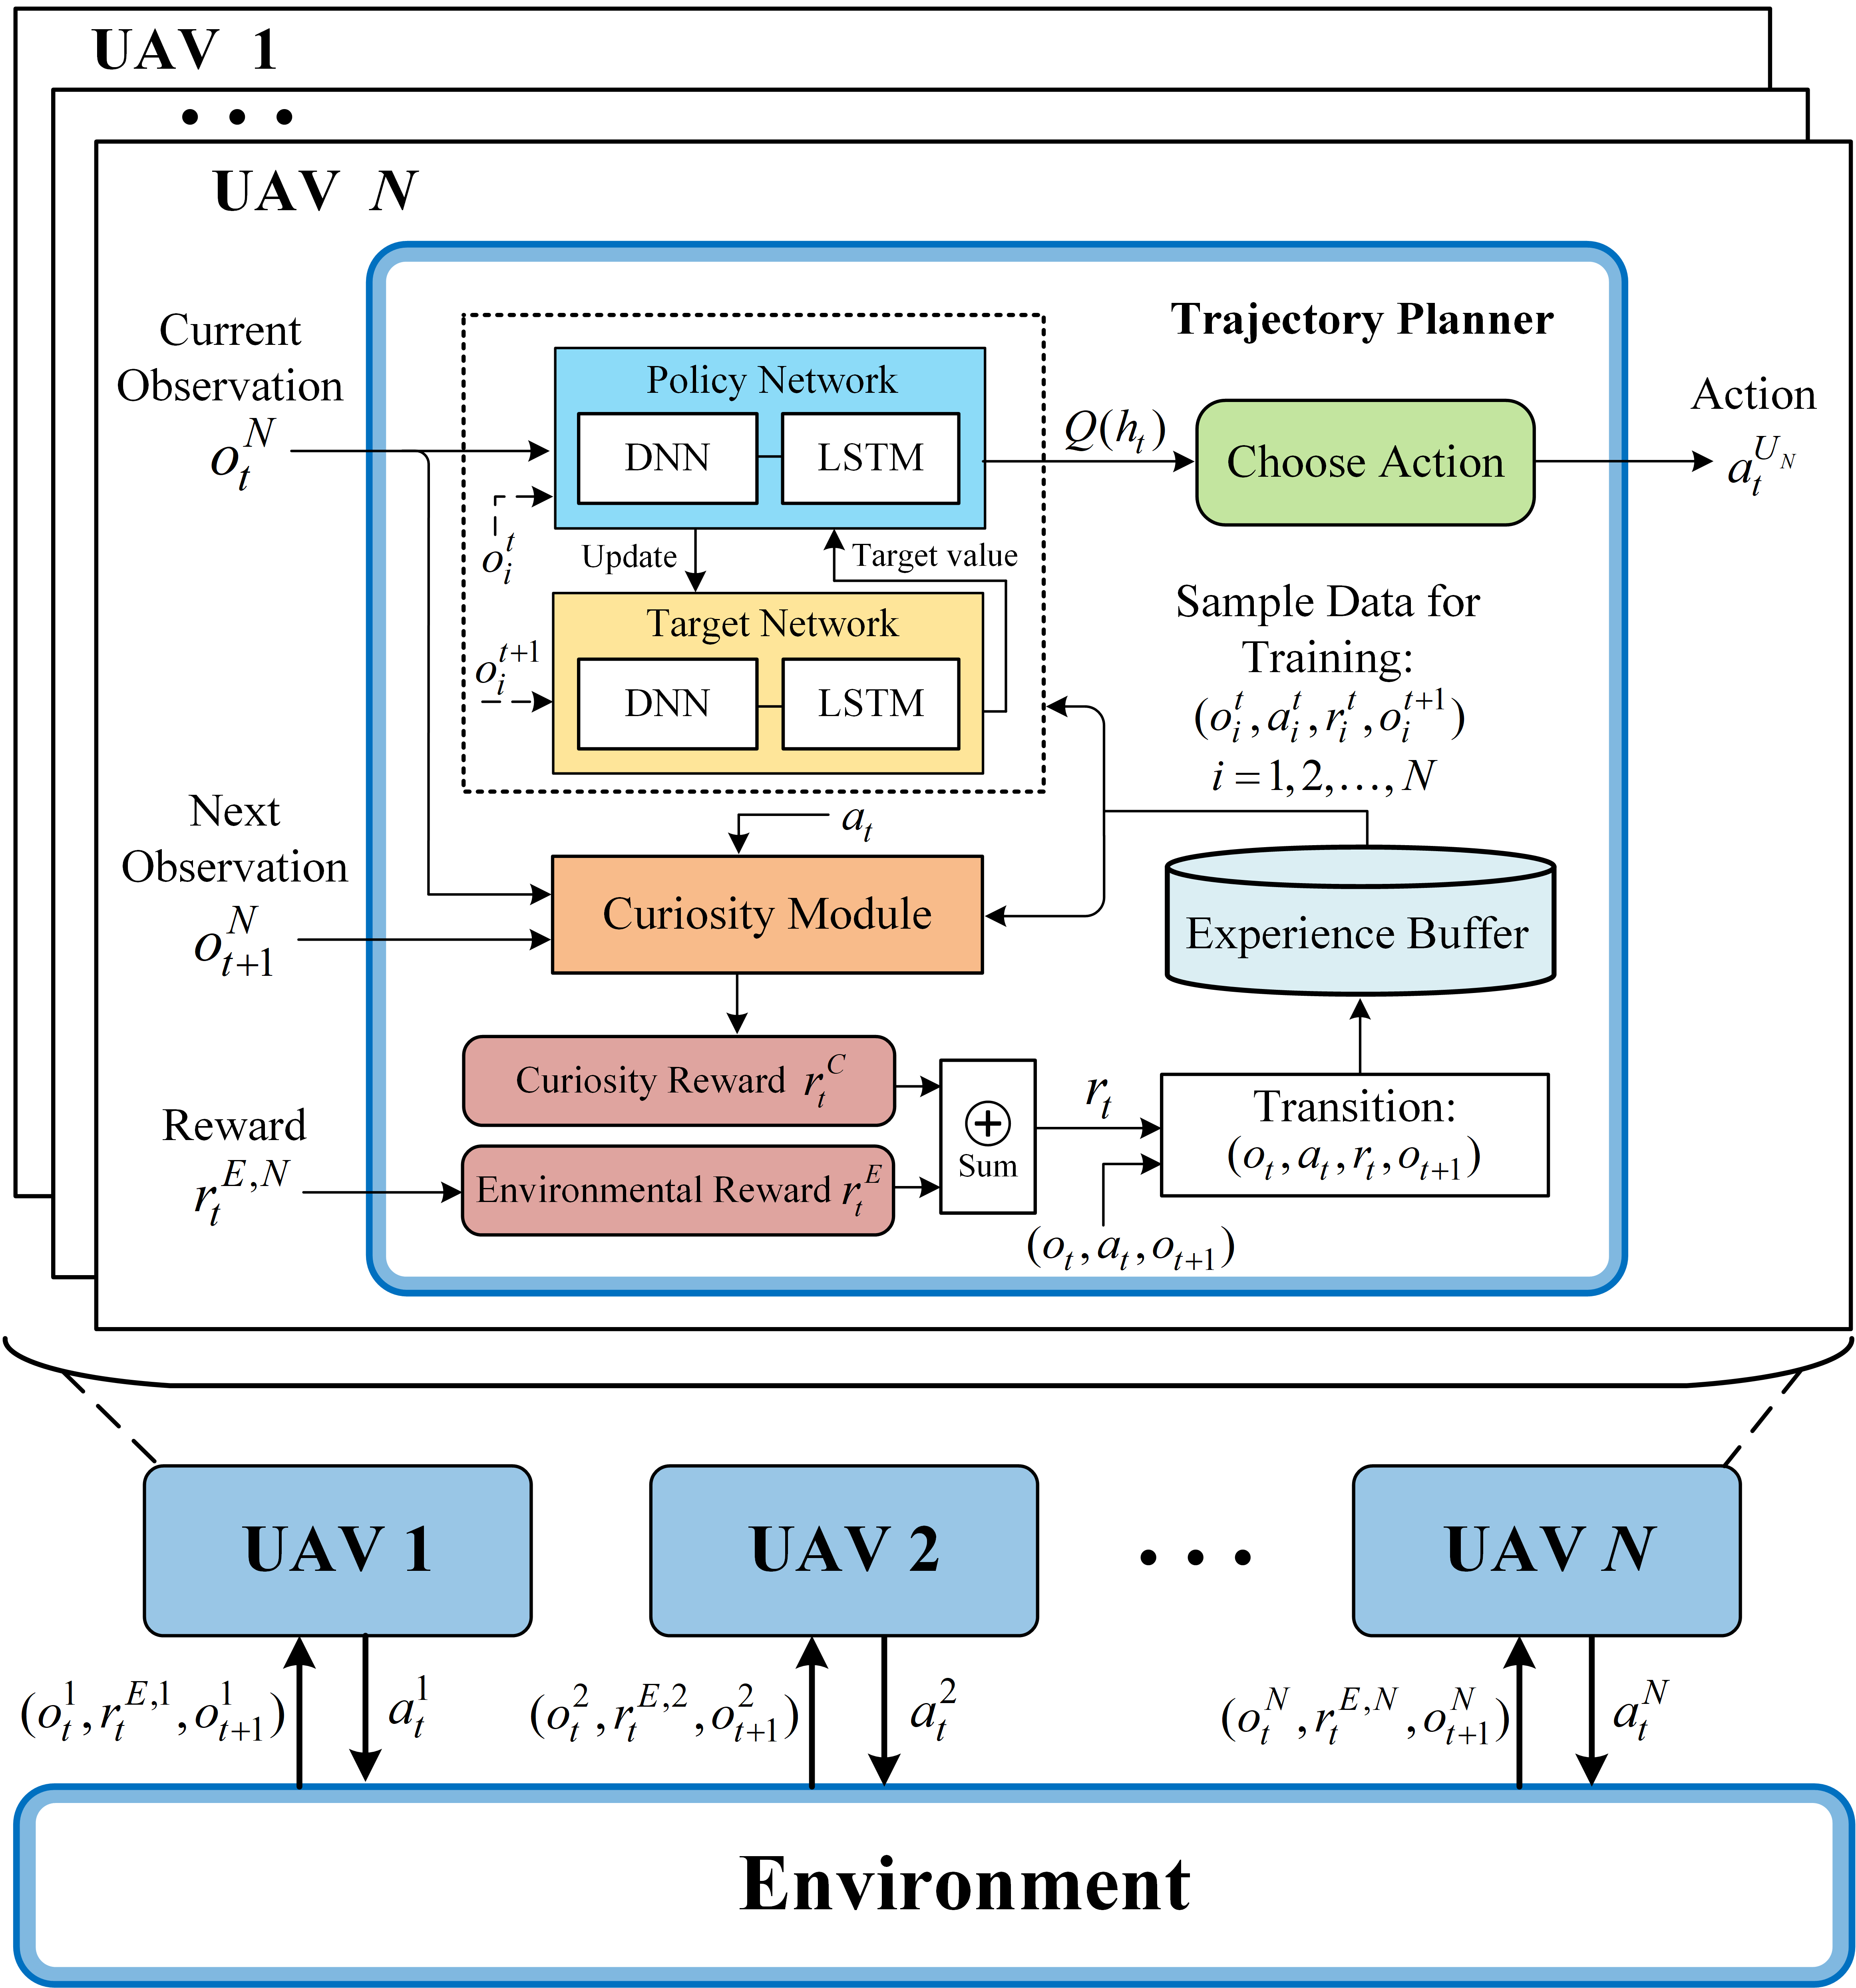
\includegraphics[width=6.75cm]{fig/Framework_ICM.png}}
\caption{The architecture of proposed CCTP algorithm.}
\label{framework}
\end{figure}
\subsection{DRQN-based reinforcement learning for data collection}
In this work, a curiosity-enhanced cooperative trajectory planning (CCTP) algorithm for multi-UAV data collection is developed. In it, a deep recurrent Q-network (DRQN) that aggregates historical observations is utilized for action policy. Then, a dual-incentive reward mechanism that integrates extrinsic environmental rewards with intrinsic curiosity reward is used for policy training, thereby enabling robust trajectory planning in partially observable and dynamically complex environments.

As shown in Fig. \ref{framework}, each agent holds a policy network that integrates a deep neural network (DNN) with a long short term memory (LSTM). The DNN extracts the features of environment from the observation input. The LSTM stores the features of previous observations and generates a feature of inferred state based on these historical observations. Lastly, an output layer estimates values of action decisions based on the feature map from LSTM. With the help of LSTM, the trajectory planner can accurately recognize the dynamically changing environment state and make precise trajectory planning. 

In the UAV agent $U_i$, the output of DNN is denoted as:
\begin{equation}\label{dnn_out}
  \phi\left(o_{t}^{i}\right)=DNN_{U_i}\left(o_{t}^{i}\right).
\end{equation}
The LSTM employs gating mechanisms to selectively store the historical inputs and outputs the feature map of inferred state based on the current and historical inputs, i.e. 
\begin{equation}\label{lstm_out}
  h^{i}_{t}=LSTM_{U_i}\left[\phi\left(o_{t}^{i}\right),h^{i}_{t-1}\right].
\end{equation}
Finally, the policy network outputs the state-action values based on the inferred state, which is denoted as $Q\left(h^{i}_{t}\right)$. For the optimal policy, the agent choose the action that has the highest estimated state-action value, i.e. 
\begin{equation}\label{action_policy}
  a^{i}_{t}=\mathop{\arg\max}\limits_{a} Q\left(h^{i}_{t}, a\right).
\end{equation}

The iteration of action value network is based on temporal difference (TD) error, i.e. 
\begin{equation}\label{q_iteration}
  L\left(\theta^{i}_{Q}\right)=\left[{r^{i}_{t}+\gamma \mathop{\max}\limits_{a'} Q\left({h^{i}_{t+1},a'}\right)-Q\left({h^{i}_{t},a^{i}_{t}}\right)}\right]^2, 
\end{equation}
where $\theta^{i}_{Q}$ is the parameter of policy network, $\gamma$ is the discount factor. As shown in Fig. \ref{framework}, the DRQN has a twin neural network structure. Policy network is deployed for trajectory planning policy and target network is deployed for calculating $Q\left({h^{i}_{t+1},a'}\right)$ to stabilize the TD error calculation. The parameters of target network is directly copied from policy network but the updating of target network is less frequent than policy network. A experiment buffer is built to store the transition $\left({o^{i}_{t}, a^{i}_{t}, r^{i}_{t}, o^{i}_{t+1}}\right)$ in every step. In each iteration, a batch of transitions with batch size $N_B$ for training policy network is randomly sampled from the buffer. 

\subsection{Intrinsic curiosity reward}
The complexity of trajectory planning increases due to the unknown and dynamically changing environment. The DRQN-based trajectory planner exhibits enhanced learning efficacy for optimal trajectory planning strategies when it explores the environment comprehensively in training process. Hence, an ICM is deployed in each agent to motivate the agent to explore the environment for the globally optimal solution by giving the agent an curiosity reward in the process of training the trajectory planner. The ICM estimates the curiosity reward based on the prediction error of the next observation which reflects the novelty of experiencing an environment state transition \cite{FHuang22}. 
%Although our reward function can encourage each UAV to collect the data, avoid the collision and fly to the destination, the reward function components of data collection and collision avoiding are still sparse that the UAV agent will not receive the reward in some areas. If the UAV agent wanders in these areas, it will not receive adequate reward for training. Hence, a curiosity module is deployed to motivate the agent to explore the environment for the globally optimal solution by giving the agent additional reward \cite{Bahloul21}. The ICM gives the additional reward based on the prediction error of the next state which reflects the novelty of experiencing an environment state transition \cite{Dubey20,FHuang22,BLi19}. 

As shown in Fig. \ref{curiosity_framework}, within the ICM deployed in the UAV agent $U_i$, a twin of neural networks extract features of input observations in two steps which are denoted as $\phi_{C}\left(o^{i}_{t}\right)$ and $\phi_{C}\left(o^{i}_{t+1}\right)$. A forward network predicts the next observation based on the current observation and conducted action, i.e.
\begin{equation}\label{icm_fwd}
  \hat{\phi_{C}}\left({o^{i}_{t+1}}\right)=f^{i}_{F}\left({o^{i}_{t}, a^{i}_{t}}\right).
\end{equation}
The curiosity reward is the prediction error of the forward network, i.e. 
\begin{equation}\label{icm_output}
  r^{i}_{C}=\left[{\hat{\phi_{C}}\left({o^{i}_{t+1}}\right)-\phi_{C}\left({o^{i}_{t+1}}\right)}\right]^{2}.
\end{equation}
The forward network is updated by the back propagation of state prediction error. With each iteration, the state prediction error under current input is minimized, leading to an attenuation of the curiosity toward previously experienced environment state transition. 

To evaluate the qualities of feature extraction networks, an inverse network is introduced to predict the action based on the observations in adjacent two steps, i.e.
\begin{equation}\label{icm_inv}
  \hat{a}^{i}_{t}=f^{i}_{I}\left({\phi_{C}\left({o^{i}_{t}}\right),\phi_{C}\left({o^{i}_{t+1}}\right)}\right).
\end{equation}
The feature extraction networks are updated together with the inverse network by the back propagation of action prediction error which is denoted as: 
\begin{equation}\label{icm_del_inv}
  \delta\left({a^{i}_{t}}\right)=L_{I}\left({a^{i}_{t}, \hat{a}^{i}_{t}}\right),
\end{equation}
where the $L_{I}$ is the loss function. For the discrete action space, a cross-entropy loss function is deployed. Finally, the $r^{i}_{C}$ is propagated to the DRQN, serving as a curiosity-driven reward. 
\begin{figure}[tbp]
\centerline{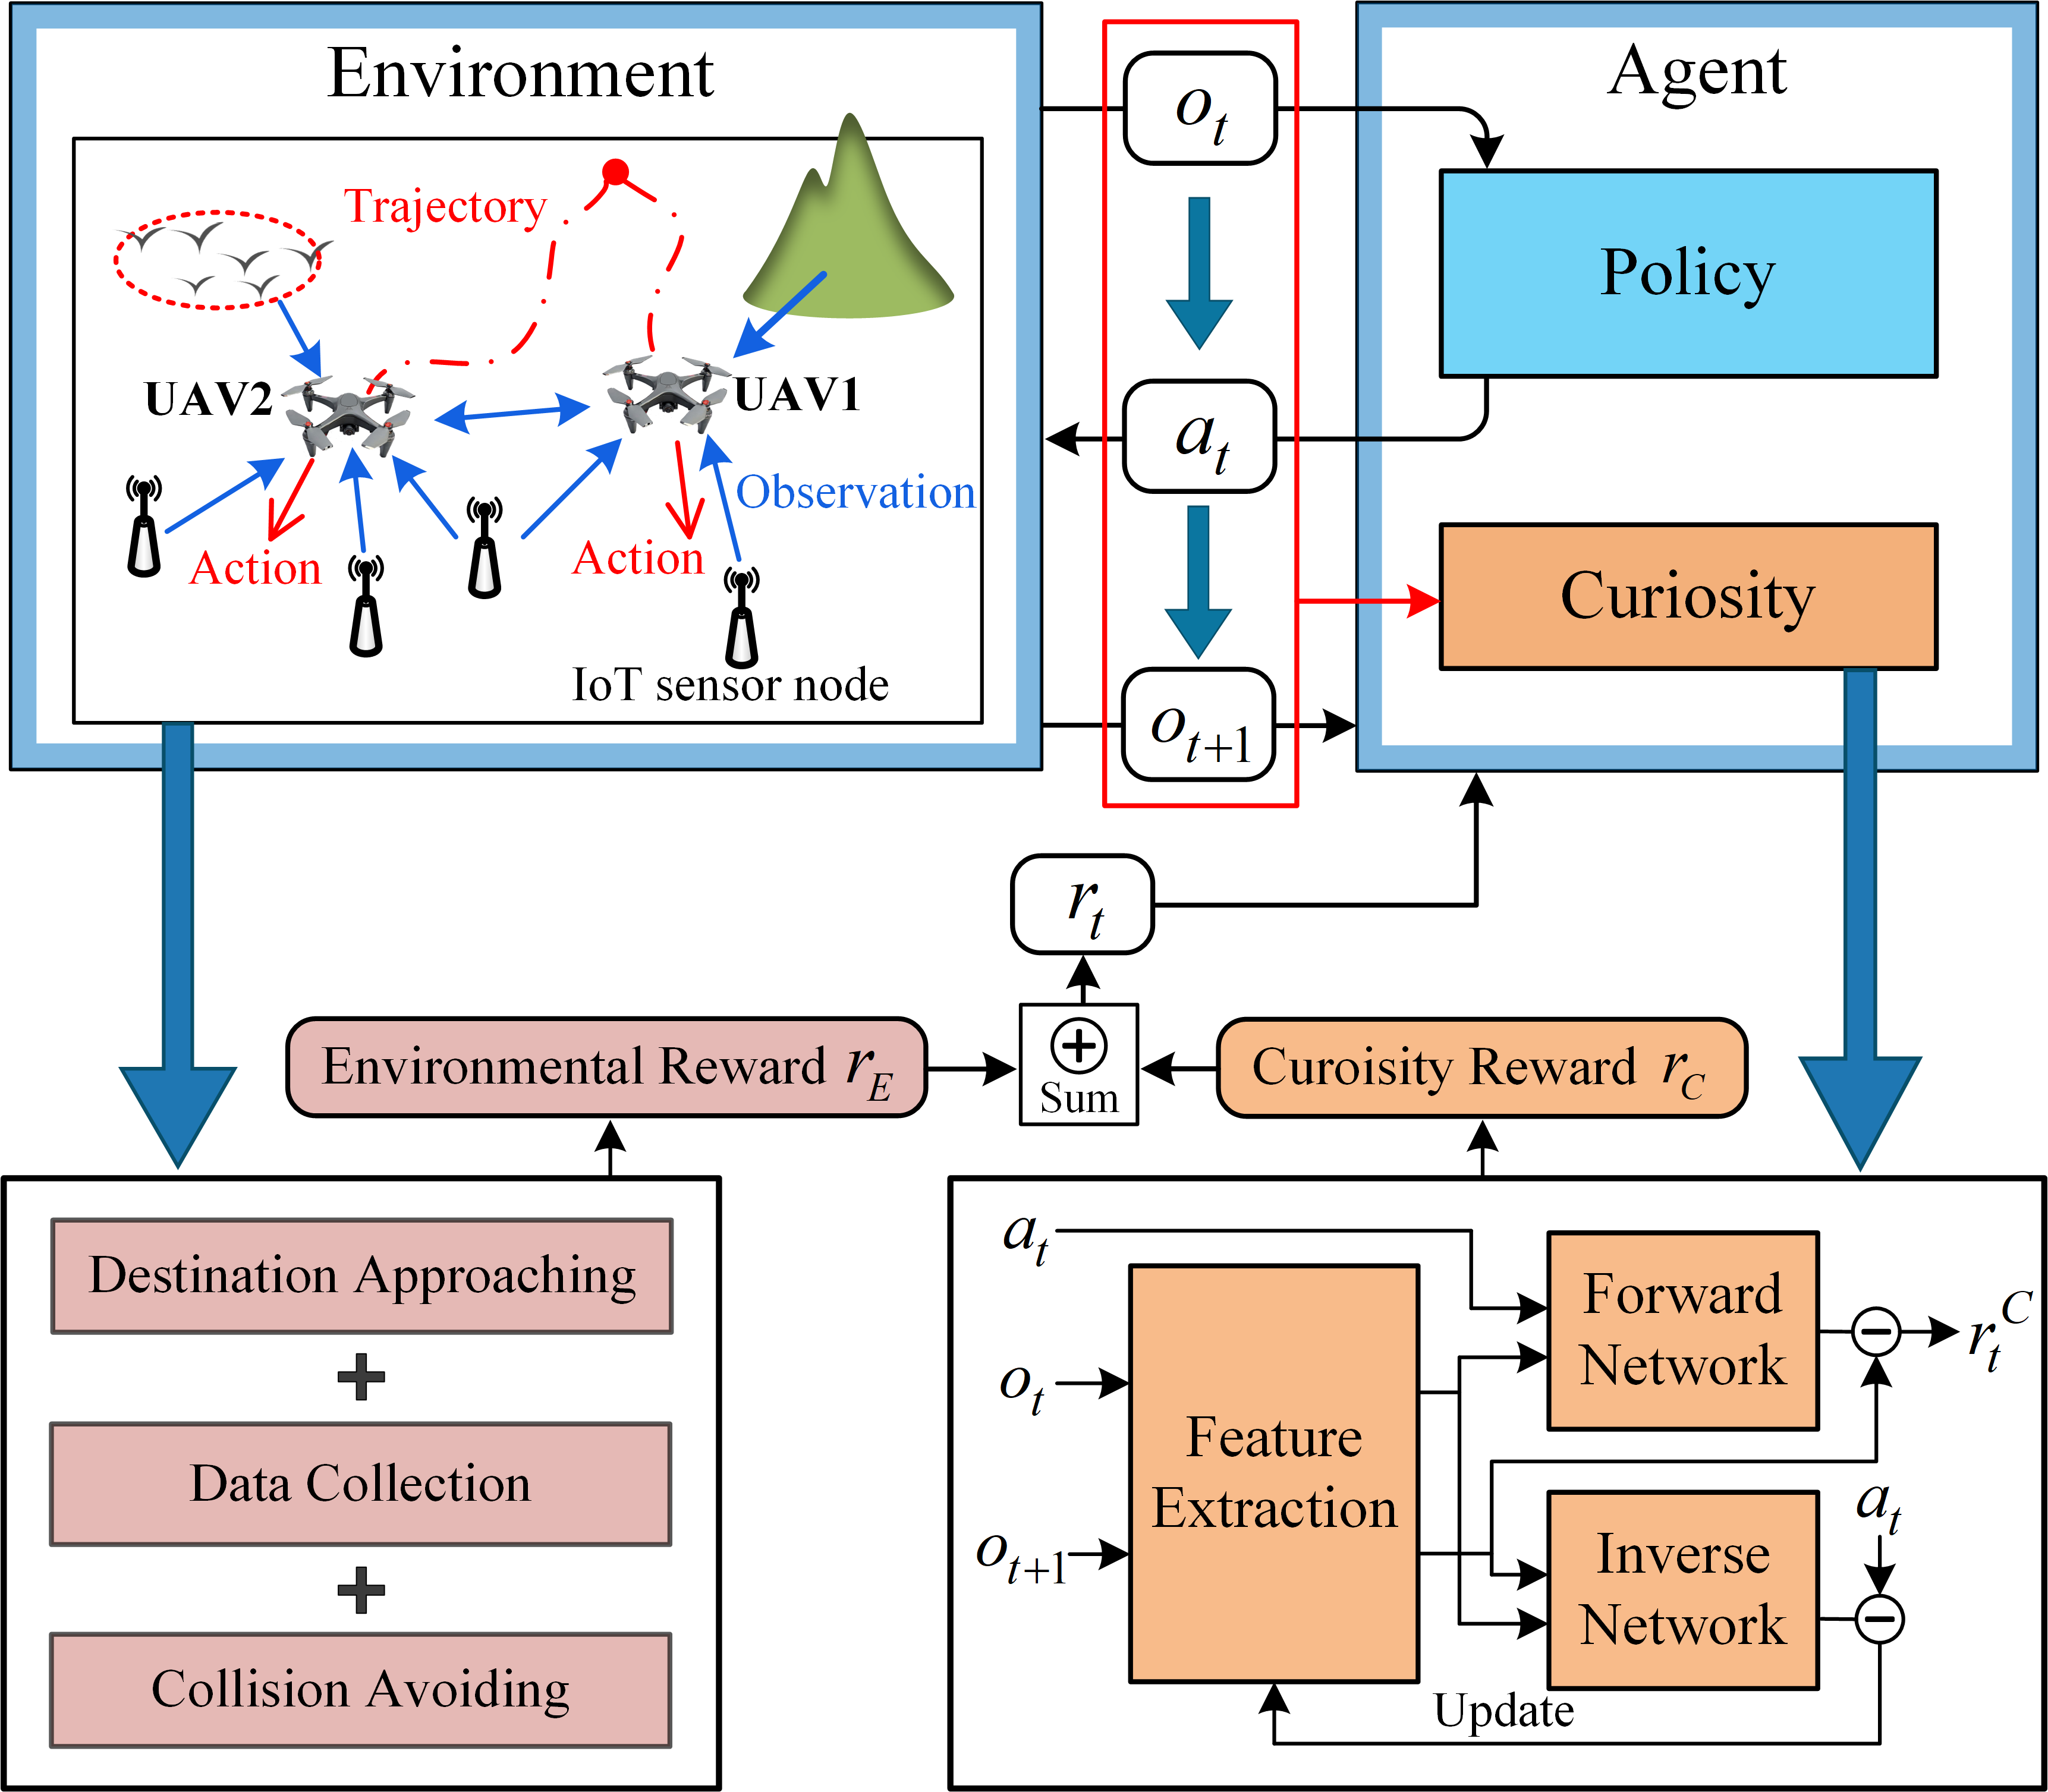
\includegraphics[width=6.9cm]{fig/Curiosity Mechanism.png}}
\caption{The framework of intrinsic curiosity reward mechanism.}
\label{curiosity_framework}
\end{figure}
\begin{table*}[tb]
	\renewcommand{\arraystretch}{1.3}
	\caption{The parameter settings for simulation.\label{parameters}}
	\centering
	\begin{tabular}{c|c|c|c|c|c}
		\hline %\hline
		\textbf{Parameter} & \textbf{Value} & \textbf{Parameter} & \textbf{Value} & \textbf{Parameter} & \textbf{Value} \\ \hline
		Flying height $H$ & 50m & Noise power $\sigma ^2$ & -90dBm & Communication range $d^{I}_{\max}$  & 50m\\ %\hline
        Flying velocity $V$ & 10m/s & Bandwidth $B$ & 1MHz & Signal transmission power $P$ & -20dBm\\ %\hline
		Channel parameters $\alpha$, $\beta$ & 10, 0.6 & Carrier frequency $f_c$ & 2.4GHz & Reward constants $K_1$, $K_2$, $K_3$ & -5, -3, -0.05  \\ %\hline 
        Reward factors $\alpha_{1}$, $\alpha_{2}$ & 0.15, 1 & Reward factors $\alpha_{3}$, $\alpha_{4}$ & 0.69, 0.115 & Scaling factor of curiosity $\beta_C$ & 1 \\ %\hline
        Learning rate of DRQN & 0.0001 & Batch size $N_B$ & 16 & Size of experience buffer $L_B$  & 80,000 \\ %\hline
        Learning rate of ICM & 0.0001 & Discount factor $\gamma$ & 0.95 & Iteration period of target network $N_T$  & 100 \\ \hline %\hline
	\end{tabular}
\end{table*}

\subsection{Environmental reward functions}
After the UAV agent conducts its action, it receives a reward as the feedback from the environment. 
%As the trajectory planning model is trained to select an action that can maximize the agent's expected cumulative reward, the configuration of reward function critically determines the action choosing policy of the trajectory planning model. 
To facilitate accomplishing data collection task while jointly optimizing the collected data amount and task completion time, the reward functions are designed appropriately. For the agent $U_i$, the received reward are described as follows: 
 
\textit{(a) Destination approaching reward:} The destination approaching reward encourages the UAV flies to the destination when no uncollected IoT node is discovered, which is denoted as: 
\begin{equation}\label{reward_1}
r^{E_1,i}_{t}=
\begin{cases}
            \alpha_{1}\left({d_{t-1}^{i,tar}-d_{t}^{i,tar}}\right), & \mbox{$o^{i}_{I}\neq\varnothing$}\\
            \alpha_{2}\left({d_{t-1}^{i,tar}-d_{t}^{i,tar}}\right), & \mbox{otherwise}
\end{cases},
\end{equation}
where $\alpha_{1}$ and $\alpha_{2}$ are scaling factors that $\alpha_{1} < \alpha_{2}$. 

\textit{(b) Data collection reward:} To encourage UAV find a shortest route to collect data, when the UAV is approaching to one node, it receives the approaching reward from the node. Meanwhile, to encourage the UAV to collect as much as data amount from IoT nodes, when the UAV finished data collection from one node, it receives the collected data amount reward. The reward from the IoT sensor node $I_j$ is denoted as: 
\begin{equation}\label{reward_2_i}
r^{i,j}_{t}=
\begin{cases}
            \alpha_{3}\left({d_{t-1}^{i,j}-d_{t}^{i,j}}\right), & \mbox{$\varphi^{I_j}_c=0$}\\
            \alpha_{4}D_{c}^{i,j}, & \mbox{$\varphi^{I_j}_c=1$}
\end{cases},
\end{equation}
where $\varphi^{I_j}_c$ is the collection state of node $I_j$ and value 1 denotes the data collection is finished, $D^{C}_{i,j}$ is the collected data amount from node $I_j$ by the UAV $U_i$ and $\alpha_{3}$, $\alpha_{4}$ are scaling factors. To jointly optimize the collection sequence and trajectory, the data collection reward $r_{E_2}$ is the sum of the reward components of the observed IoT nodes, i.e.
\begin{equation}\label{reward_2}
r^{E_2,i}_{t}=\sum_{j\in \mathcal{I}_{i}}r^{i,j}_{t},
\end{equation} 
where $\mathcal{I}_{U_{i}}$ is the set of IoT sensor nodes that observed by the UAV $U_i$. 

\textit{(c) Collision reward:} This reward assumes a negative scalar value to penalize suboptimal actions causing UAV's proximity to obstacles and adjacent UAVs, i.e.
\begin{equation}\label{reward_3}
r^{E_3,i}_{t}=
\begin{cases}
            K_1, & \mbox{$d^{i,m}_{t}<d_{\min}^{B}$}\\
            K_2, & \mbox{$d^{i,n}_{t}<d^{U}_{\min}$}\\
            K_3, & \mbox{$d^{i,n}_{t}>d^{U}_{\max}$}\\
            0, & \mbox{otherwise}
\end{cases},
\end{equation}
where $K_1$, $K_2$, $K_3$ are negative constants, $d^{i,m}_{t}$ is the distance between UAV $U_i$ and the surface of nearest obstacle $B_m$, $d_{\min}^{B}$ is the minimum distance to the obstacle surface, $d^{i,n}_{t}$ is the distance between $U_i$ and the nearest adjacent UAV $U_n$, $d^{U}_{\min}$ is the minimum safety distance between adjacent UAVs and $d^{U}_{\max}$ is the maximum communication maintaining distance between adjacent UAVs. 

Finally, the external environment reward is the sum of these components, i.e.
\begin{equation}\label{ext_reward}
  r^{E,i}_{t}=r^{E_1,i}_{t}+r^{E_2,i}_{t}+r^{E_3,i}_{t}.
\end{equation}
The proposed algorithm combines the extrinsic environmental reward with the intrinsic curiosity reward to formulate the agent’s feedback after action execution, i.e.
\begin{equation}\label{tol_reward}
  r^{i}_{t}=r^{E,i}_{t}+\beta_C \cdot r^{C,i}_{t},
\end{equation}
where $\beta_C$ is the scaling factor of curiosity reward. 
%\begin{figure*}[htbp]
%\centerline{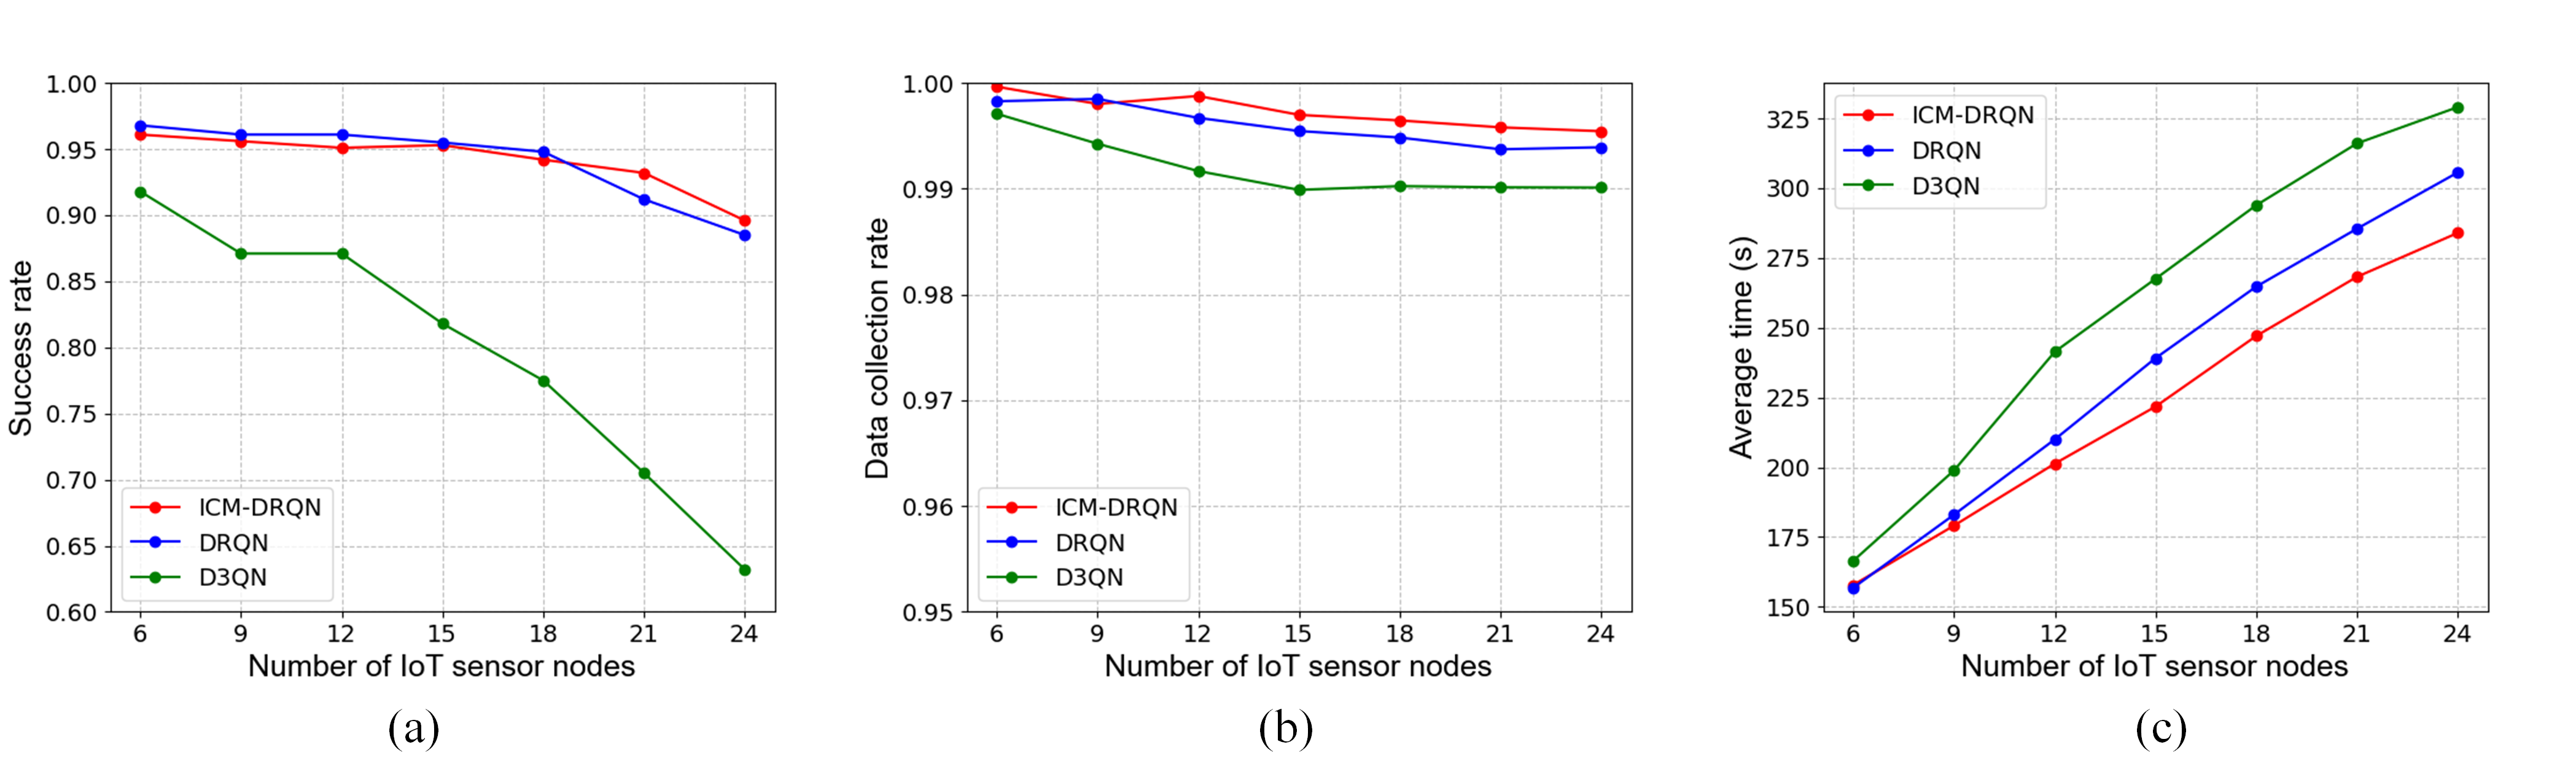
\includegraphics[width=16cm]{fig/perf_iot.png}}
%\caption{The result of performance test in different numbers of IoT sensor nodes: (a) Success rate; (b) Data collection rate; (c) Average time in seconds.}
%\label{perf_iot}
%\end{figure*}
%\begin{algorithm}[htb]	
%	Initialize the policy network $\theta_Q$, the target network $\theta '_Q$ by $\theta '_Q\gets \theta_Q$ and the experience buffer $\mathbf{B}$\;
%	\For{$episode=1,2,\cdots,E$}
%	{
%		Initialize the environment\;
%        Clear the memory of LSTM\;
%		Receive the first observation $o_{t}$\;
%		\While{$terminal \neq True$}
%		{
%			Choose an action $a_{t}\gets\pi\left({o_{t}}\right)$\;
%            Apply action $a_{t}$ to the environment, obtain next observation $o_{t+1}$, reward $r_{t}$ and task finish flag $terminal$\;
%            Push transition $(o_t, a_t, r_t, o_{t+1})$ into $\mathbf{B}$\;
%            Randomly sample $N_B$ transitions $(o^{t}_i, a^{t}_i, r^{t}_i, o^{t+1}_{i})$ from $\mathbf{B}$\;
%            Update policy network $\theta_Q$ using equation (\ref{q_iteration}) every $N_P$ decision processes\;
%            Update target network $\theta '_Q$ by $\theta '_Q\gets \theta_Q$ every $N_{T}$ iterations\;
%            Update ICM using equation (\ref{icm_output}) and (\ref{icm_del_inv}) by $(o_t, a_t, o_{t+1})$\;
%            Clear the memory of LSTM every $L$ steps\;
%            $o_t \gets o_{t+1}$
%		}
%	}
%	\caption{training process of ICM-DRQN}\label{alg1}
%\end{algorithm}
%\subsection{Training}
%In the initial stage of training, the agent makes trajectory planning decisions by its randomly initialized policy network and target network. The policy network iterates by the training data sampled from experience buffer while the agent is exploring the environment and collecting transition experiences. When the number of iterations is sufficient to make policy network convergent, the training process ends and the trained DRQN model can be applied to trajectory planning in any environment. The ICM iterates at every trajectory control decision step as it reflects the novelty of the state transition experience. 
%\begin{table}[tb]
%	\renewcommand{\arraystretch}{1.3}
%	\caption{The hyper-parameter settings for simulation environment.\label{hyperparameters_env}}
%	\centering
%	\begin{tabular}{c|c}
%		\hline %\hline
%		\textbf{Hyper-parameter} & \textbf{Value} \\ \hline
%		Flying height $H$ & 50m \\ \hline
%        Flying velocity $V$ & 10m/s \\ \hline
%		Maximum task time & 400s \\ \hline  
%		Noise power $\sigma ^2$ & -90dBm \\ \hline
%        Bandwidth $B$ & 1MHz \\ \hline
%        Carrier frequency $f_c$ & 2.4GHz \\ \hline
%        Communication range $R^C$  & 50m \\ \hline
%        Signal transmission power $P$ & -20dBm \\ \hline
%        Maximum data amount in each node $D_{\max}$  & 6MB \\ \hline
%	\end{tabular}
%\end{table}
%\begin{table}[tb]
%	\renewcommand{\arraystretch}{1.3}
%	\caption{The hyper-parameter settings for our algorithm.\label{hyperparameters_alg}}
%	\centering
%	\begin{tabular}{|c|c|}
%		\hline %\hline
%		\textbf{Parameter} & \textbf{Value}  \\ \hline
%		Learning rate of DRQN & 0.0001 \\ \hline
%        Learning rate of ICM & 0.0001 \\ \hline
%		Batch size $N_B$ & 16  \\ \hline
%        Discount factor $\gamma$ & 0.95 \\ \hline  
%		Size of experience buffer $L_B$  & 80,000 \\ \hline
%        Memory length of LSTM layer $L$  & 10 \\ \hline
%        Iteration period of target network $N_T$  & 100 \\ \hline
%		%\hline  		
%	\end{tabular}
%\end{table}
\section{Experiment Results}\label{result}
The multi-UAV data collection simulation is realized in Python platform and the neural networks are constructed using PyTorch. The environment region is a $1000\times1000$m\textsuperscript{2} area, where 3 UAVs jointly collect the data of IoT sensor nodes. The positions of IoT sensor nodes and obstacles are stochastically assigned. The data storage capacity in IoT nodes is randomly configured with an upper bound of 6MB. The obstacles are set as cylinders with radius randomly assigned within the interval of 1m to 5m. Furthermore, the moving obstacles have stochastically generated motion trajectories. The time limitation of data collection task is 400s. The neural networks in DRQN is formed by 2 fully-connected layers and one LSTM layer. Each layer has 256 neurons. The neural networks in ICM is formed by 3 fully-connected layers. Each layer in forward network and feature extraction network has 256 neurons and each layer in inverse network has 512 neurons. The remaining parameters are specified as detailed in Table \ref{parameters}. 

For comparison, two benchmark algorithms are used: (1) One is DRQN algorithm that is same with our algorithm but without curiosity reward, which is marked as ``DRQN''. (2) The other is the D3QN-based algorithm proposed in \cite{XWang22}, which is marked as ``D3QN''. For performance evaluation, some metrics are defined: (1) Success rate, which is the ratio of the number of successful tasks to the number of all data collection tasks. The successful task is that all the UAVs arrive at the destination. (2) Data collection rate, which is the ratio of the amount of collected data to the amount of all the stored data in successful tasks. (3) Average time, which is the average task completion time in successful tasks. 
%\begin{figure*}[htbp]
%	\centering
%	\subfigure[\quad Success rate]{
%		\centering
%		
\includegraphics[width=4.8cm]{fig/perf_ob/SR.png}
%		\label{fig_perf_ob_sr}
%	}
%	\subfigure[\quad Data collection rate]{
%		\centering 
%		
\includegraphics[width=4.8cm]{fig/perf_ob/DCR.png}
%		\label{fig_perf_ob_dcr}
%	}
%	\subfigure[\quad Average time]{		
%		\raggedright
%		
\includegraphics[width=4.8cm]{fig/perf_ob/AT.png}	
%		\label{fig_perf_ob_at}
%	}		
%	\caption{Data collection trajectory planning performance in different number of moving obstacles: (a) Success rate; (b) Data collection rate; (c) Average time. Note that the average time is in seconds. \label{perf_ob}} 				
%\end{figure*}
%\begin{figure*}[htbp]
%\centerline{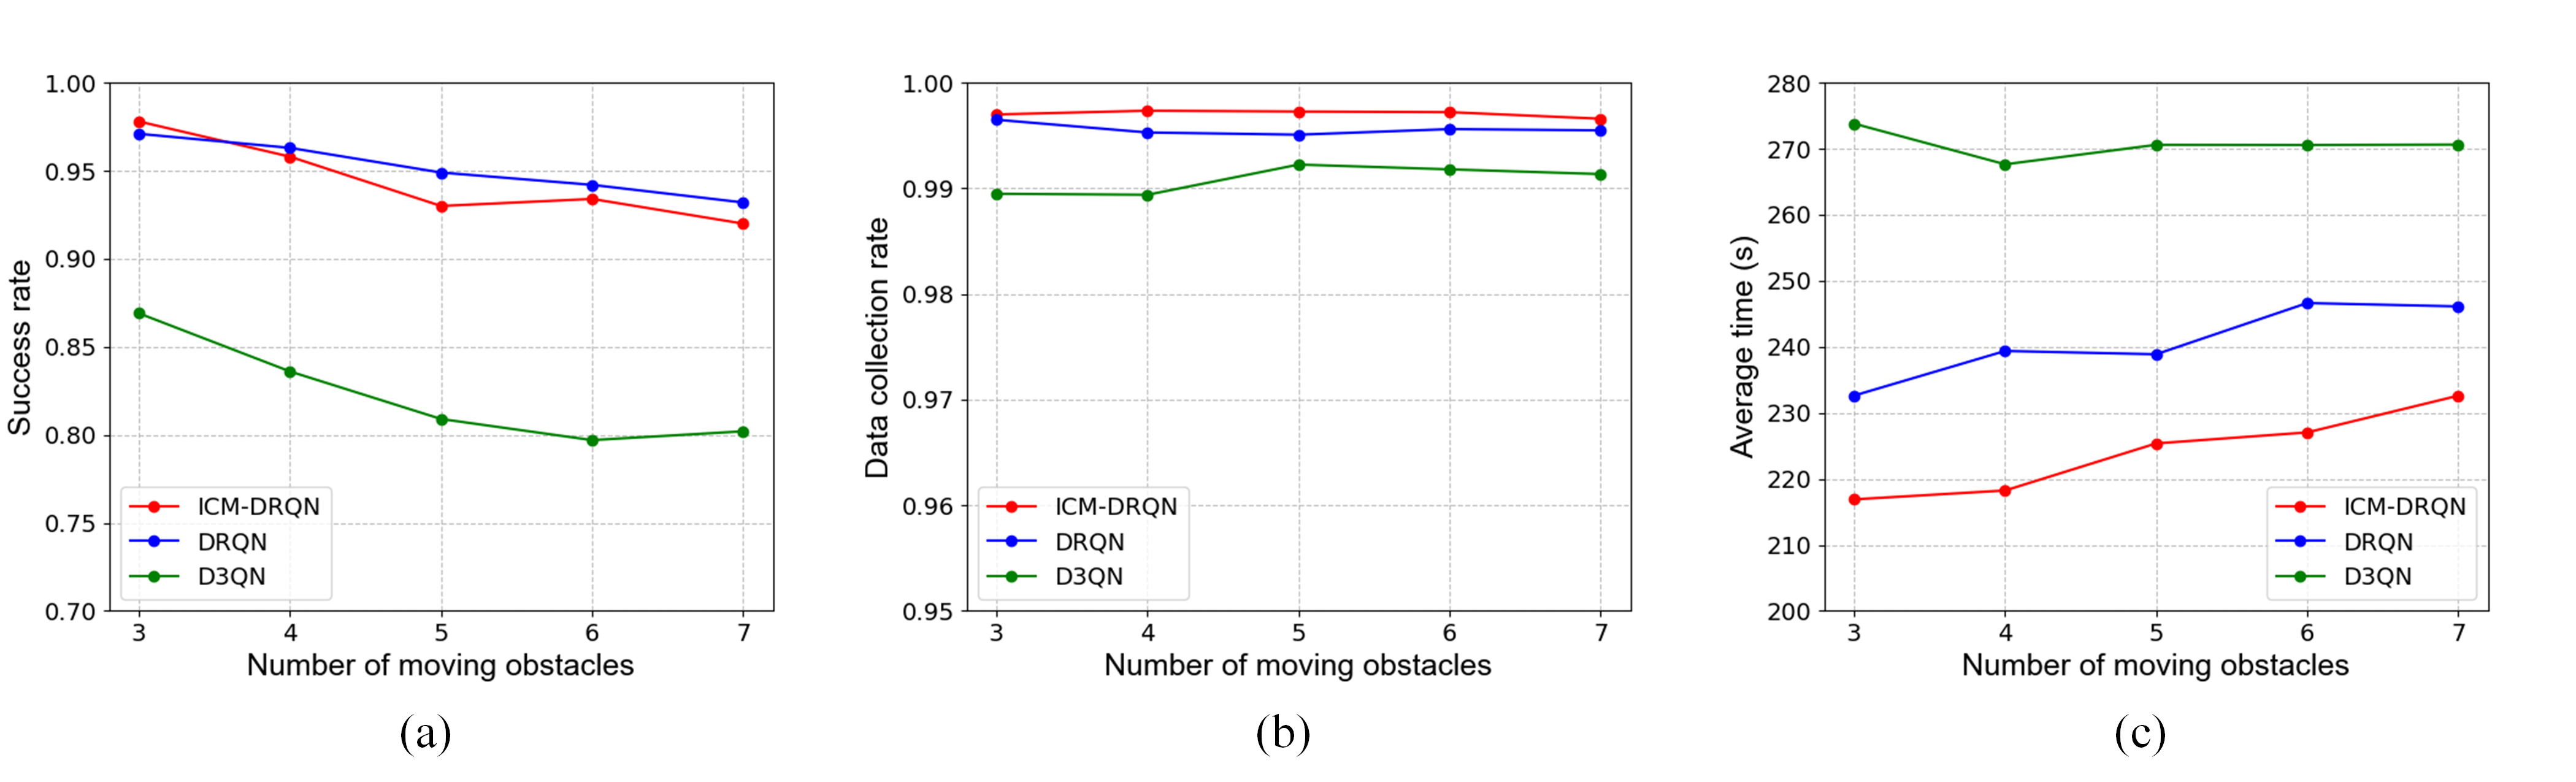
\includegraphics[width=16cm]{fig/perf_ob.png}}
%\caption{The result of performance test in different numbers of moving obstacles: (a) Success rate; (b) Data collection rate; (c) Average time in seconds.}
%\label{perf_ob}
%\end{figure*} 
\begin{figure}[htb]
\centerline{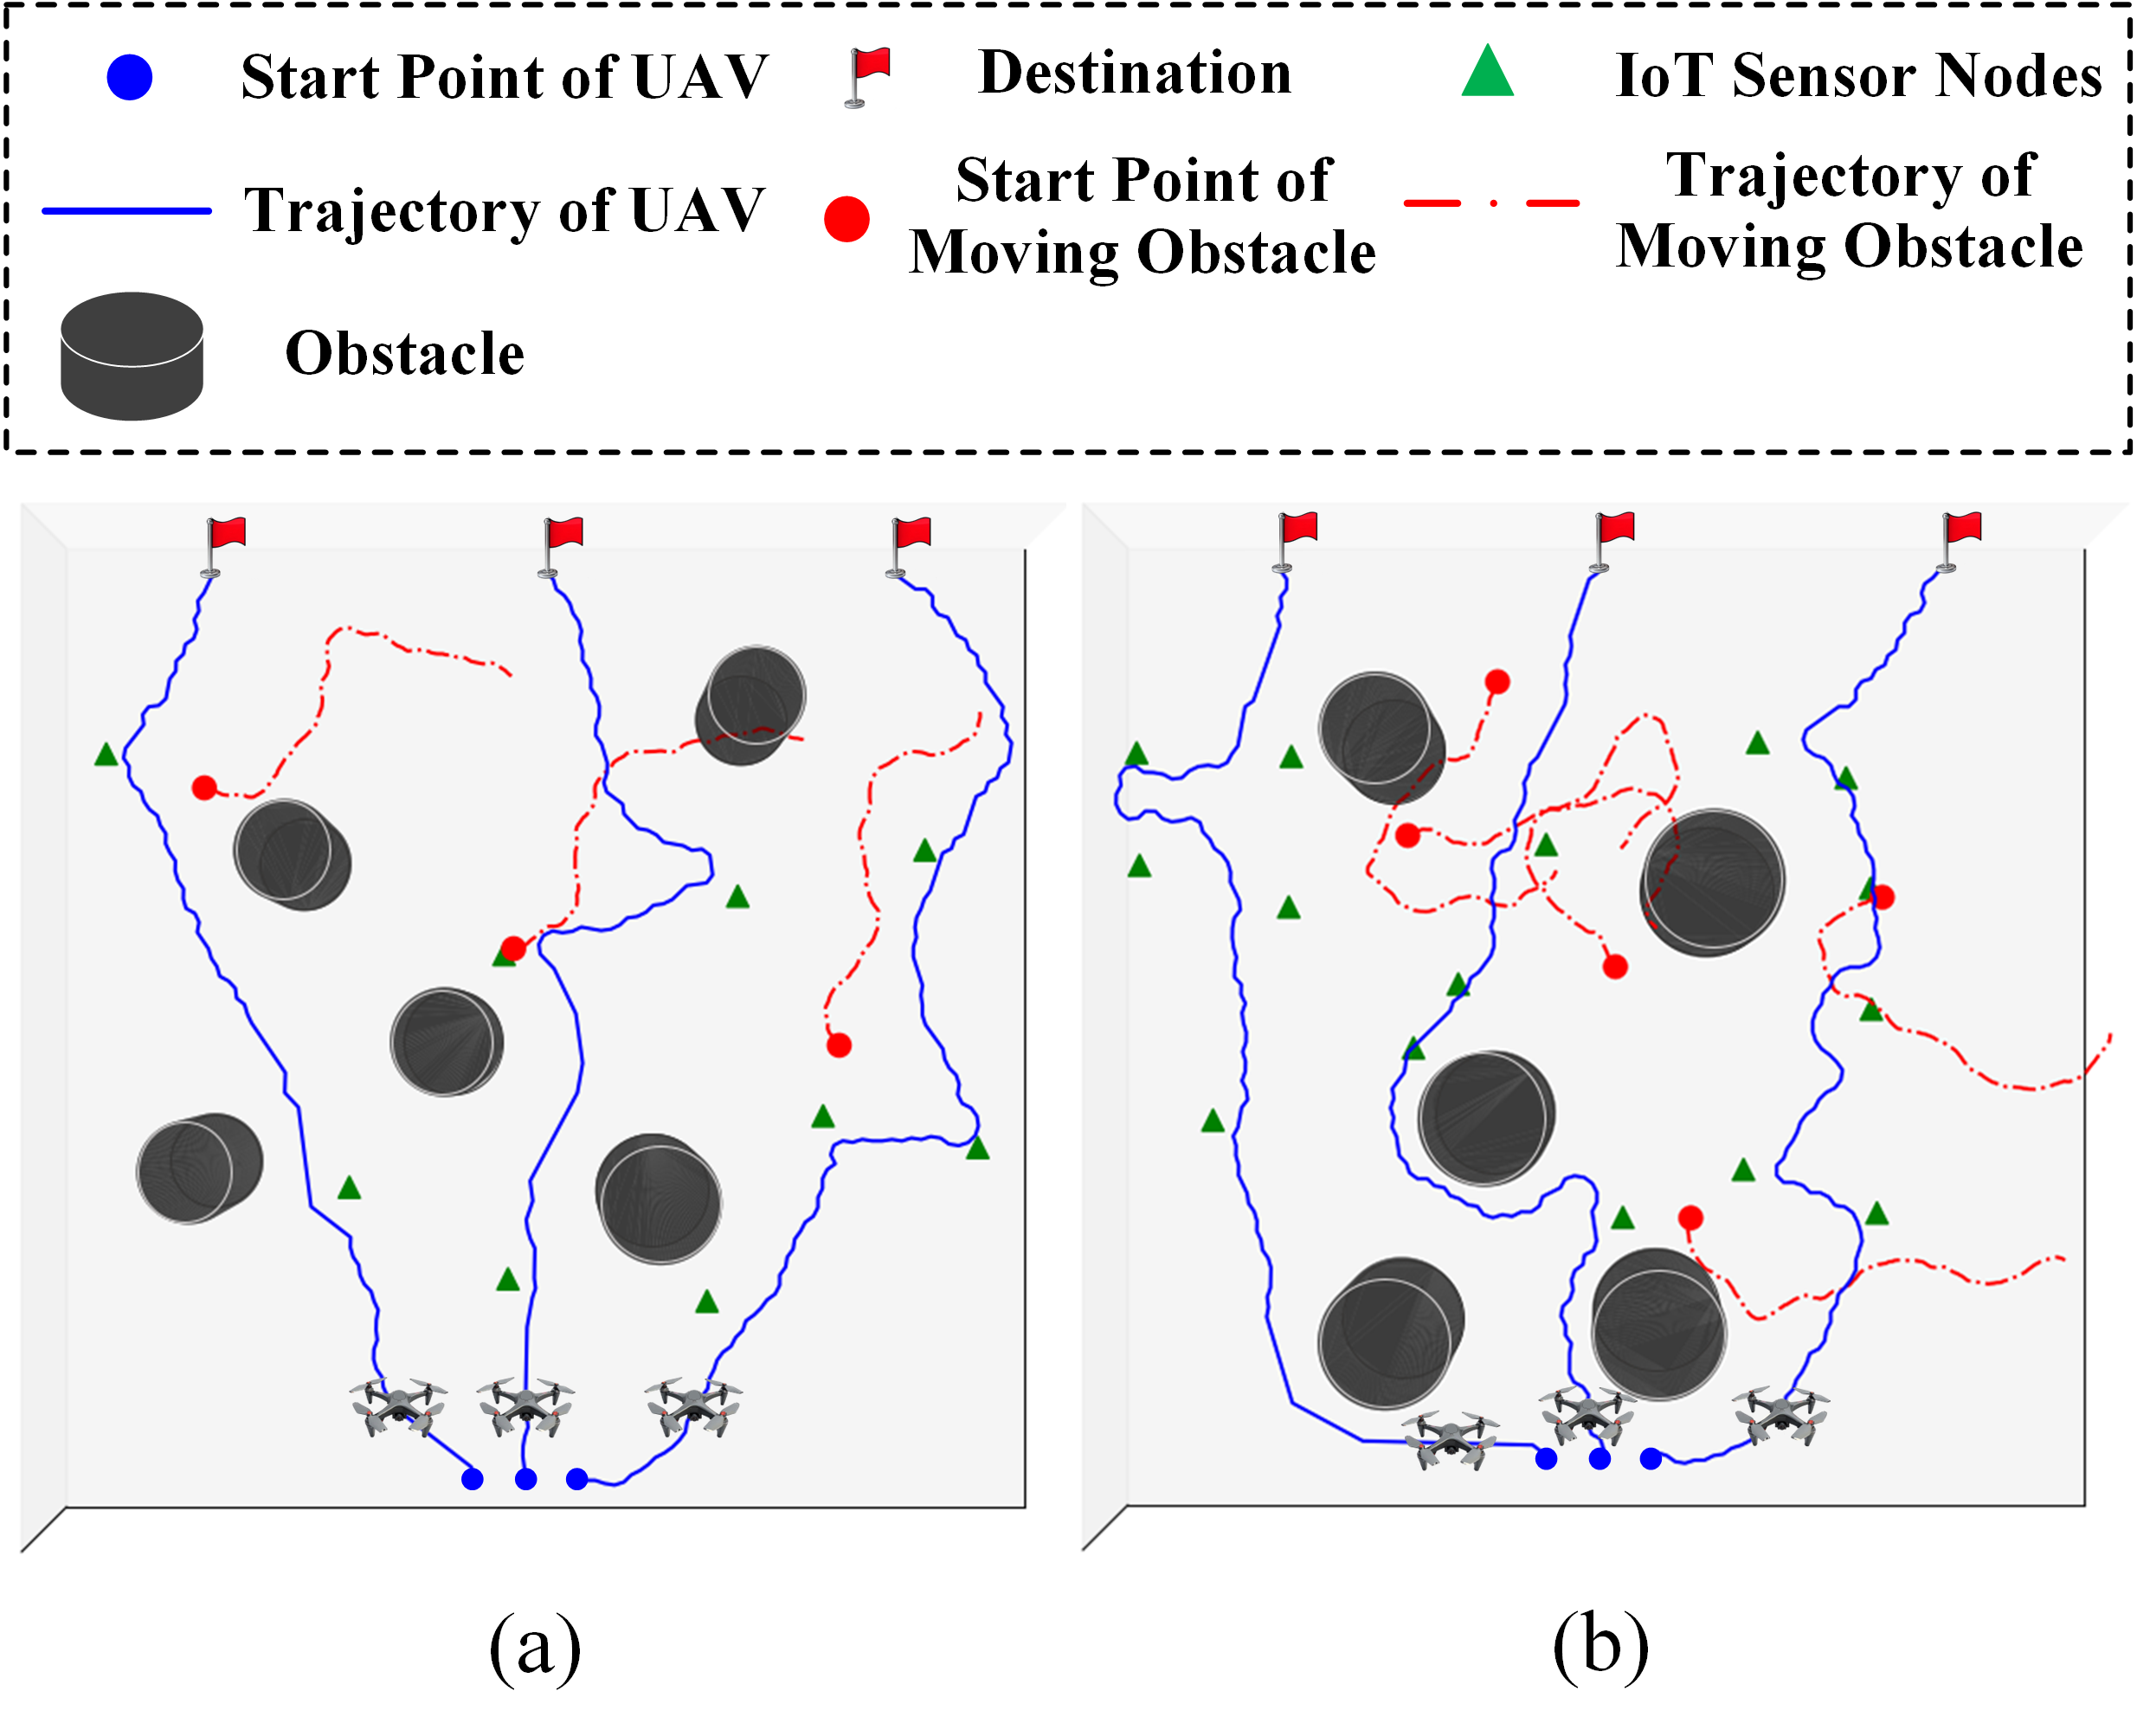
\includegraphics[width=6.75cm]{fig/trajectory.png}}
\caption{The UAV trajectories in different numbers of IoT sensor nodes: (a) 9 IoT sensor nodes; (b) 15 IoT sensor nodes.}
\label{traj}
\end{figure}
\begin{figure*}[htb]
	\centering
	\subfigure[\quad Success rate]{
		\centering
		
\includegraphics[width=4.15cm]{fig/perf_iot/SR.png}
		\label{fig_perf_iot_sr}
	}
	\subfigure[\quad Data collection rate]{
		\centering 
		
\includegraphics[width=4.15cm]{fig/perf_iot/DCR.png}
		\label{fig_perf_iot_dcr}
	}
    \subfigure[\quad Collision rate]{
		\centering 
		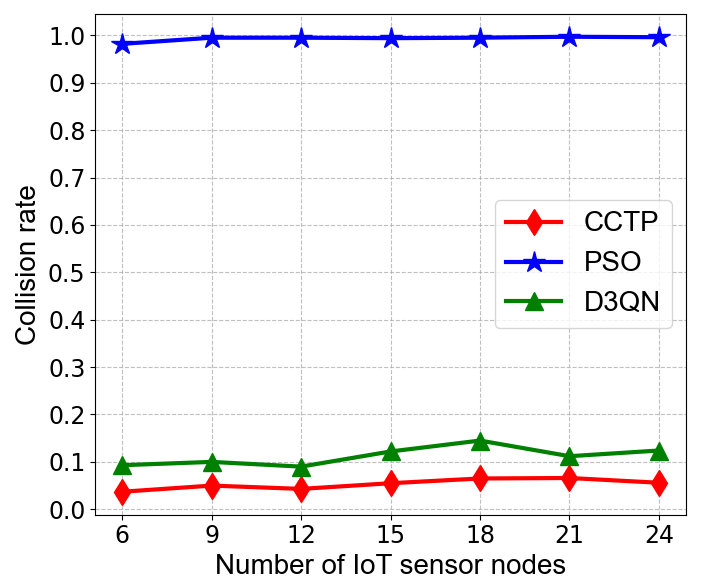
\includegraphics[width=4.15cm]{fig/perf_iot/CR.png}
		\label{fig_perf_iot_cr}
	}
	\subfigure[\quad Average time]{		
		\raggedright
		
\includegraphics[width=4.15cm]{fig/perf_iot/AT.png}	
		\label{fig_perf_iot_at}
	}
    \subfigure[\quad Success rate]{
		\centering
		
\includegraphics[width=4.15cm]{fig/perf_ob/SR.png}
		\label{fig_perf_ob_sr}
	}
	\subfigure[\quad Data collection rate]{
		\centering 
		
\includegraphics[width=4.15cm]{fig/perf_ob/DCR.png}
		\label{fig_perf_ob_dcr}
	}
    \subfigure[\quad Collision rate]{
		\centering 
		
\includegraphics[width=4.15cm]{fig/perf_ob/CR.png}
		\label{fig_perf_iot_cr}
	}
	\subfigure[\quad Average time]{		
		\raggedright
		
\includegraphics[width=4.15cm]{fig/perf_ob/AT.png}	
		\label{fig_perf_ob_at}
	}		
	\caption{Data collection and collision avoidance performance: (a) - (d) number of IoT sensor nodes changes; (e) - (h) number of moving obstacles varies. \label{perf}} 				
\end{figure*}
\subsection{Data collection performance}
We conduct the test in which the UAVs finish the data collection in varying numbers of IoT sensor nodes to verify the data collection performance of our algorithm. The environment in this test has 5 static obstacles, 5 moving obstacles and 6 to 24 IoT sensor nodes. 
As shown in Fig. \ref{traj}, each UAV has a smooth trajectory, even though its work load increases. 

The performance results are shown in Fig. \ref{perf}. The success rate of CCTP is similar to that of DRQN, but the success rate of D3QN is about 15\% lower than that of the other two algorithms when there are 15 IoT sensor nodes. The reason is that the reward function of D3QN is only related to the collected data, making D3QN can not find the best sequence and trajectory to the IoT sensor nodes and its flight time exceeds the maximum time when the number of IoT sensor nodes increases. All the algorithms have a data collection rate of over 99\% and the data collection rate of CCTP is 1\% higher than that of DRQN and 7\% higher than that of D3QN when there are 15 IoT sensor nodes. The reason is that the CCTP has stable collection capability when the IoT node distribution is scattered. The average time of CCTP is 6.68\% shorter than that of DRQN and 15.94\% shorter than that of D3QN when there are 18 IoT sensor nodes, because the intrinsic curiosity reward in CCTP promotes each UAV agent to find a shorter path. 

\subsection{Obstacle avoiding performance}
The obstacle avoiding performance is tested in the environment with varying numbers of moving obstacles because avoiding moving obstacles is more difficult than avoiding static obstacles. The environment in this test has 5 static obstacles, 15 IoT sensor nodes and 3 to 7 moving obstacles. The performance results are shown in Fig. \ref{perf}. The success rate of CCTP is similar to that of DRQN and 12\% higher than that of D3QN. As all the algorithms exhibit average time that is far from the maximum, the main contribution to the failure of task is collision. Hence, the obstacle avoiding ability of CCTP is similar to DRQN and the obstacle avoiding ability of D3QN is lower than that of the other two algorithms. Although the UAVs have to handle increasing moving obstacles, all the algorithms have the steady data collection rate compared to Fig. \ref{perf} (b) in 15 IoT sensor nodes. The average time of CCTP is 5.50\% shorter than that of DRQN and 15.10\% shorter than that of D3QN when there are 7 moving obstacles. The similar average time performance of obstacle avoiding test to the data collection test proves that the CCTP has the enhancement on trajectory planning ability compared to DRQN and D3QN. 

\section{Conclusion}\label{conclusion}
This paper developes a curiosity-enhanced cooperative trajectory planning (CCTP) algorithm to address the multiple UAV data collection in complex and dynamic environment. The DRQN-based trajectory control policy enables effective decision-making for UAVs in partially observable and dynamic environment. The dual-incentive reward mechanism enhances the performance of the trained policy. Experiment results show that the proposed algorithm has better performance on planning a shorter flight trajectory to collect most of data in IoT sensor nodes. As the flight control of UAV is in horizonal plane in this paper, our future work will consider realizing the 3-D path planning. 

\begin{thebibliography}{00}
%\bibitem{Xiao22} Z. Xiao et al., ``A survey on millimeter-wave beamforming enabled UAV communications and networking,'' in IEEE Communications Surveys \& Tutorials, vol. 24, no. 1, pp. 557-610, Firstquarter 2022. 
\bibitem{YLi23} Y. Li, W. Liang, W. Xu et al., ``Data Collection Maximization in IoT-Sensor Networks via an Energy-Constrained UAV,'' IEEE Transactions on Mobile Computing, vol. 22, no. 1, pp. 159-174, 1 Jan. 2023.
\bibitem{JLi20}J. Li, H. Zhao, H. Wang et al., ``Joint Optimization on Trajectory, Altitude, Velocity, and Link Scheduling for Minimum Mission Time in UAV-Aided Data Collection,'' IEEE Internet of Things Journal, vol. 7, no. 2, pp. 1464-1475, Feb. 2020. 
\bibitem{MLi23} M. Li, X. Liu and H. Wang, ``Completion Time Minimization Considering GNs' Energy for UAV-Assisted Data Collection,'' IEEE Wireless Communications Letters, vol. 12, no. 12, pp. 2128-2132, Dec. 2023. 
    
\bibitem{TWang22} T. Wang, Z. Liu, L. Xu et al., ``An efficient and robust UAVs’ path planning approach for timely data collection in wireless sensor networks," in Proc. 2022 IEEE Wireless Communications and Networking Conference (WCNC), Austin, TX, USA, 2022, pp. 914-919. 

\bibitem{TWang24} T. Wang, X. Fu, A. Guerrieri, ``Joint resource scheduling and flight path planning of UAV-assisted IoTs in response to emergencies,'' Computer Networks, Vol. 253, 110731, 2024. 
\bibitem{ZDai23} Z. Dai, C. H. Liu, R. Han et al., ``Delay-Sensitive Energy-Efficient UAV Crowdsensing by Deep Reinforcement Learning,'' IEEE Transactions on Mobile Computing, vol. 22, no. 4, pp. 2038-2052, 1 April 2023. 
\bibitem{XXie23} X. Xie, C. Xu, Z. Zhang et al., ``Real-Time Traffic Based Air-Ground Cooperation for Vehicular Data Collection Using DRL Approach,'' GLOBECOM 2023 - 2023 IEEE Global Communications Conference, Kuala Lumpur, Malaysia, 2023, pp. 6910-6915. 
    
\bibitem{Rahim23} S. Rahim, L. Peng, S. Chang et al., ``On collaborative multi-UAV trajectory planning for data collection,'' Journal of Communications and Networks, vol. 25, no. 6, pp. 722-733, Dec. 2023. 
\bibitem{XWang22} X. Wang, M. C. Gursoy, T. Erpek et al., ``Learning-based UAV path planning for data collection with integrated collision avoidance,'' IEEE Internet of Things Journal, vol. 9, no. 17, pp. 16663-16676, Sept. 2022. 
\bibitem{Khodaparast21} S. S. Khodaparast, X. Lu, P. Wang et al., ``Deep reinforcement learning based energy efficient multi-UAV data collection for IoT networks,'' IEEE Open Journal of Vehicular Technology, vol. 2, pp. 249-260, 2021.
\bibitem{Bayerlein21} H. Bayerlein, M. Theile, M. Caccamo et al., ``Multi-UAV Path Planning for Wireless Data Harvesting With Deep Reinforcement Learning,'' IEEE Open Journal of the Communications Society, vol. 2, pp. 1171-1187, 2021. 
    
\bibitem{ZWei22} Z. Wei, M. Zhu, N. Zhang et al., ``UAV-assisted data collection for Internet of things: a Survey,'' IEEE Internet of Things Journal, vol. 9, no. 17, pp. 15460-15483, Sept. 2022. 
\bibitem{LZhang24} L. Zhang, W. Yi, H. Lin et al., ``An Efficient Reinforcement Learning-Based Cooperative Navigation Algorithm for Multiple UAVs in Complex Environments,'' IEEE Transactions on Industrial Informatics, vol. 20, no. 10, pp. 12396-12406, Oct. 2024. 
\bibitem{LZhang24_2} L. Zhang, J. Peng, W. Yi et al., ``A State-Decomposition DDPG Algorithm for UAV Autonomous Navigation in 3-D Complex Environments,'' IEEE Internet of Things Journal, vol. 11, no. 6, pp. 10778-10790, 15 March15, 2024. 
%\bibitem{Cheng23} N. Cheng et al., ``AI for UAV-assisted IoT applications: a comprehensive review,'' in IEEE Internet of Things Journal, vol. 10, no. 16, pp. 14438-14461, Aug. 2023. 

\bibitem{YLi23} Y. Li, W. Liang, W. Xu et al., ``Data collection maximization in IoT-sensor networks via an energy-constrained UAV,'' IEEE Transactions on Mobile Computing, vol. 22, no. 1, pp. 159-174, Jan. 2023.

\bibitem{LLiu22}L. Liu, K. Xiong, J. Cao et al., "Average AoI Minimization in UAV-Assisted Data Collection With RF Wireless Power Transfer: A Deep Reinforcement Learning Scheme," IEEE Internet of Things Journal, vol. 9, no. 7, pp. 5216-5228, 1 April1, 2022. 


\bibitem{MSun21} M. Sun, X. Xu, X. Qin et al., ``AoI-energy-aware UAV-assisted data collection for IoT networks: a deep reinforcement learning method,'' IEEE Internet of Things Journal, vol. 8, no. 24, pp. 17275-17289, Dec. 2021. 
\bibitem{Nguyen22} K. K. Nguyen, T. Q. Duong, T. Do-Duy et al., ``3D UAV trajectory and data collection optimisation via deep reinforcement learning,'' IEEE Transactions on Communications, vol. 70, no. 4, pp. 2358-2371, April 2022. 
\bibitem{HQi24} H. Qi, M. Wu, Z. Zhang et al., ``Trajectory design for multi-UAV-enabled wireless powered communication networks: a multi-agent DRL approach,'' Proc. 2024 IEEE Wireless Communications and Networking Conference (WCNC), Dubai, United Arab Emirates, 2024, pp. 1-6. 

\bibitem{XFu25}X. Fu and S. Kang, "Deep Reinforcement Learning-Based Collaborative Data Collection in UAV-Assisted Underwater IoT," IEEE Sensors Journal, vol. 25, no. 1, pp. 1611-1626, 1 Jan.1, 2025. 
\bibitem{KWei22}K. Wei, K. Huang, Y. Wu et al., "High-Performance UAV Crowdsensing: A Deep Reinforcement Learning Approach," IEEE Internet of Things Journal, vol. 9, no. 19, pp. 18487-18499, 1 Oct.1, 2022, 
%\bibitem{Hourani14} A. Al-Hourani, S. Kandeepan and S. Lardner, ``Optimal LAP altitude for maximum coverage,'' in IEEE Wireless Communications Letters, vol. 3, no. 6, pp. 569-572, Dec. 2014.
\bibitem{MLi22} M. Li, S. He and H. Li, ``Minimizing mission completion time of UAVs by jointly optimizing the flight and data collection trajectory in UAV-enabled WSNs,'' IEEE Internet of Things Journal, vol. 9, no. 15, pp. 13498-13510, Aug. 2022. 
%\bibitem{Bahloul21}S. N. Bahloul and Y. Mahmoudi, ``Rainbow-RND: a value-based algorithm augmented with intrinsic curiosity,'' in Proc. 2021 International Conference on Information Systems and Advanced Technologies (ICISAT), Tebessa, Algeria, 2021, pp. 1-5. 
\bibitem{FHuang22} F. Huang, W. Li, J. Cui et al., ``Unified curiosity-driven learning with smoothed intrinsic reward estimation,'' Pattern Recognition, Vol. 123, p. 108352, 2022. 
%\bibitem{Dubey20} R. Dubey, T. L. Griffiths, ``Understanding exploration in humans and machines by formalizing the function of curiosity,'' in Current Opinion in Behavioral Sciences, Vol. 35, 2020, pp. 118-124. 
%\bibitem{BLi19} B. Li, T. Lu, J. Li, N. Lu, Y. Cai and S. Wang, ``Curiosity-driven exploration for off-policy reinforcement learning methods,'' in Proc. 2019 IEEE International Conference on Robotics and Biomimetics (ROBIO), Dali, China, 2019, pp. 1109-1114. 
\end{thebibliography}

\end{document}
